\chapter{Results and Discussion}\label{chap:results}

\section{Chapter Overview}\label{sec:results_overview}

This chapter is in two parts. Part~I, in
Section~\ref{sec:results_fer}, presents the \ac{FER} module on \ac{DAiSEE}
\cite{gupta_daisee_2016}. Part~II, in
Section~\ref{sec:results_adapt_part}, presents the adaptation
module in a Gymnasium-compatible synthetic tutoring environment.
The two parts use different protocols and are interpreted
separately. The main \ac{RL} experiments use simulator-derived affect
states (\texttt{USE\_REAL\_FER=False}) and do not quantify
end-to-end webcam-based tutoring.

\section{\ac{FER} Module Results on \ac{DAiSEE}}\label{sec:results_fer}

\subsection{Experimental Standardization}\label{sec:results_fer_standardization}

Prior \ac{FER} work on \ac{DAiSEE} evaluates models under inconsistent
conditions. Papers vary in preprocessing pipeline, frame count,
class-balancing strategy, loss function, and evaluation metric, and
several of these choices are not reported explicitly in the source
papers. A direct numerical comparison between two published
results is therefore unreliable. Any observed gap may reflect data
preparation rather than model design, and the information needed
to reproduce a published result is not always present.

To remove this confound, one standardised preprocessing and
evaluation pipeline was designed and applied to every architecture
in this chapter. The 24-frame sampling rule, per-frame normalisation, the official \ac{DAiSEE} splits, and the evaluation metrics are identical across runs. Every model was
retrained from scratch under this pipeline. Architectural and
training differences therefore explain any performance gap reported
below, not preprocessing differences. The single-label formulation
predicts one dominant class per clip with a softmax head and a
cross-entropy or focal cross-entropy loss; the multi-label
formulation predicts four independent binary labels with a sigmoid
head and a binary cross-entropy loss. The two are evaluated with
different metrics and are not compared numerically as if they
solved the same task.

\subsection{Single-Label Formulation}\label{sec:results_fer_singlelabel}

Single-label classification was evaluated first to test whether one
dominant label per clip could represent learner affect.
Table~\ref{tab:fer_singlelabel_results} reports each architecture
retrained under the standardised pipeline, with its source paper
cited inline.

\begin{table}[H]
\centering
\footnotesize
\caption{Single-label results on the \ac{DAiSEE} test split under the
standardised pipeline.}
\label{tab:fer_singlelabel_results}
\setlength{\tabcolsep}{4pt}
\begin{tabular}{p{4.8cm}lccccl}
\toprule
\textbf{Architecture} & \textbf{Loss / Sampling} & \textbf{Frames} &
\textbf{Macro F1} & \textbf{Accuracy} & \textbf{Inspired From} \\
\midrule
ResNet50 + \ac{BiLSTM} + Temp.\ Attn          & Focal CE / bal.\ CSV    & 16 & 0.311 & 0.702 & \cite{asaju_adaptive_2022,asaju_affects_2021} \\
ResNet50 + 2-\ac{BiLSTM} + Temp.\ Attn        & Focal CE / bal.\ CSV    & 24 & 0.271 & 0.581 & \cite{asaju_adaptive_2022} \\
ShuffleNetV2 + \ac{BiLSTM} + Temp.\ Attn      & Focal CE / OS           & 16 & 0.266 & 0.631 & \cite{aly_revolutionizing_2025} \\
ShuffleNetV2 + \ac{SE} + 2-\ac{BiLSTM} + Temp.\ Attn & Focal CE / bal.\ CSV  & 24 & 0.269 & 0.651 & \cite{aly_revolutionizing_2025} \\
\ac{HOG} + \ac{LBP} + \ac{SVM} (handcrafted baseline)   & RBF \ac{SVM} / bal.\ weights & 8  & 0.214 & 0.750 & --- \\
ResNet50 features + \ac{SVM} (frozen baseline) & RBF \ac{SVM} / bal.\ weights & 16 & 0.229 & 0.759 & \cite{he_resnet_2016} \\
\bottomrule
\end{tabular}
\end{table}

The strongest single-label run reaches accuracy $0.702$ and Macro
F1 $0.311$. Its per-label F1 is $0.834$ on engagement but $0.126$,
$0.161$, and $0.122$ on boredom, confusion, and frustration. Every
single-label deep model reproduces this pattern, and the \ac{SVM}
baselines do so more extremely: they collapse to predicting
engagement on almost every clip and score zero F1 on the three
minority labels while still reaching $0.75$ accuracy. High
accuracy on \ac{DAiSEE} indicates collapse to the dominant class rather
than detection of all four states. The single-label head also
cannot represent that a learner is simultaneously engaged and
confused, which is required by the adaptation module.
Figure~\ref{fig:fer_single_vs_multi} contrasts matched
architectures under both formulations.

\begin{figure}[H]
    \centering
    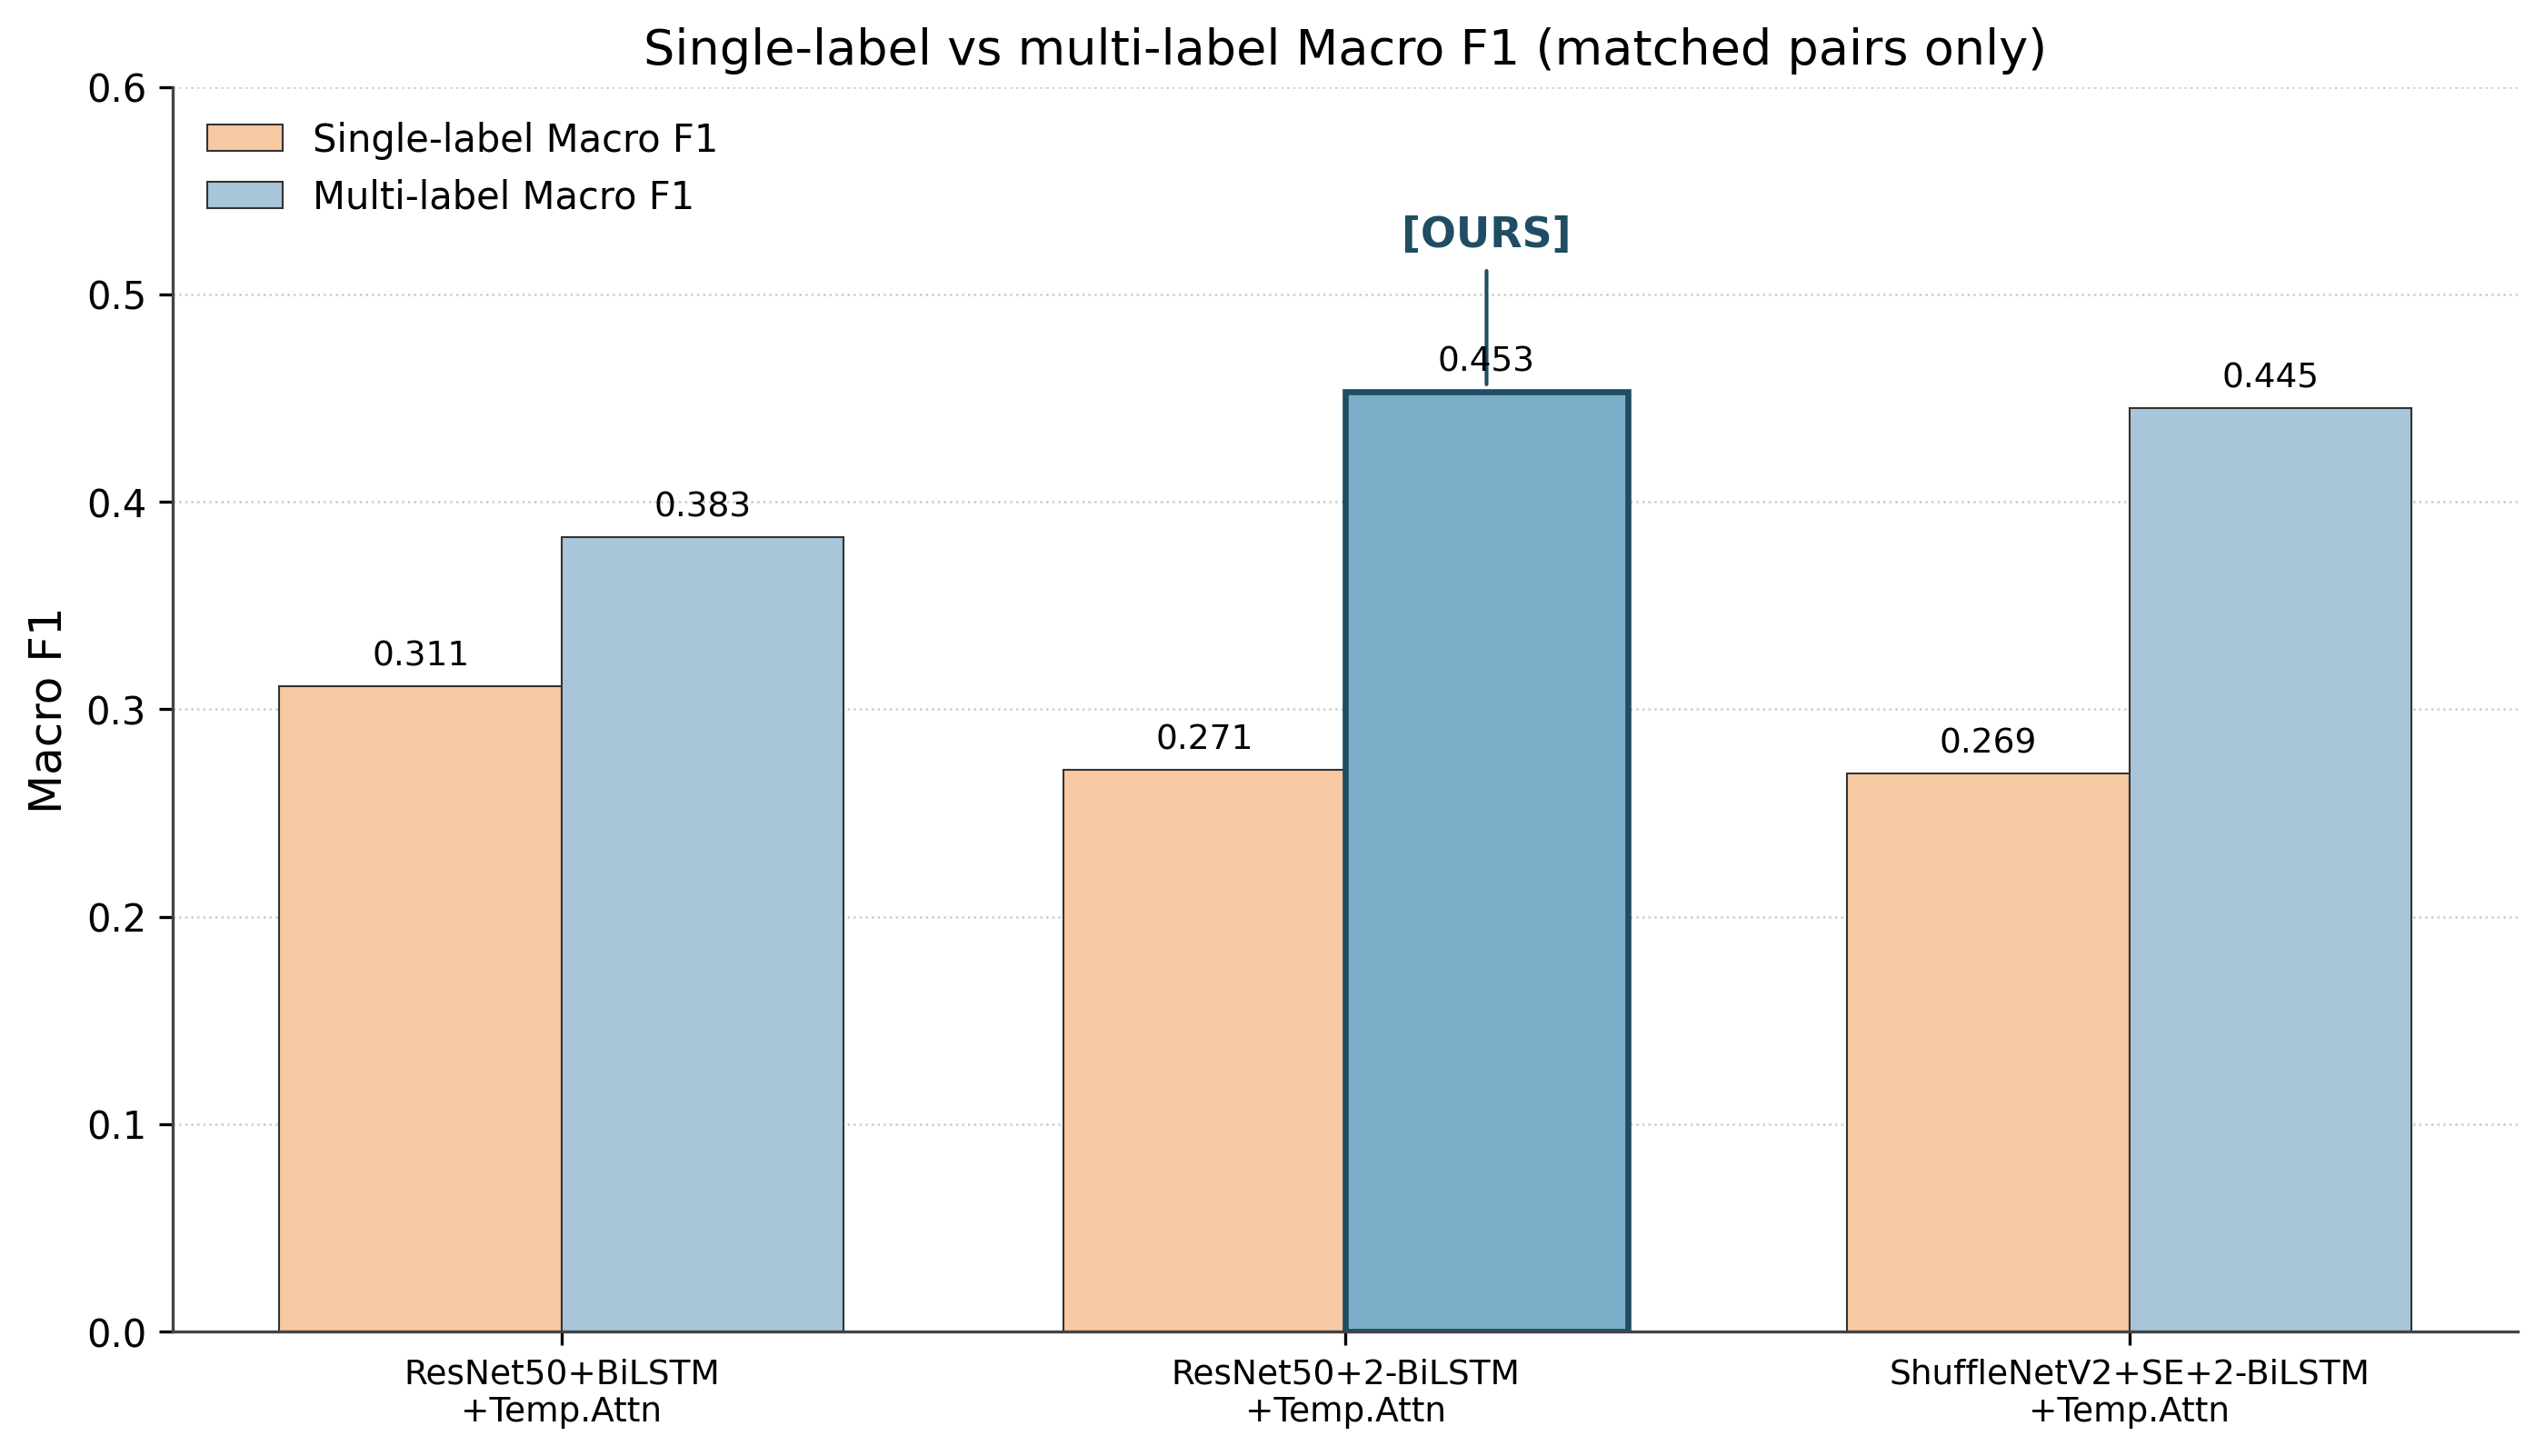
\includegraphics[width=0.92\textwidth]{Figures/fer_single_vs_multi_2.png}
    \caption{Macro F1 of architectures evaluated under both
    single-label and multi-label formulations. The proposed model is marked \textbf{[OURS]}.}
    \label{fig:fer_single_vs_multi}
\end{figure}

\subsection{Multi-Label Formulation}\label{sec:results_fer_multilabel}

Table~\ref{tab:fer_multilabel_results} reports the multi-label
architectures retrained under the standardised pipeline.
``WRS'' denotes a WeightedRandomSampler; ``OS-CSV'' denotes
fixed-multiplier oversampling
(Eng.~$\times 1$, Bor.~$\times 2$, Con.~$\times 3$, Fru.~$\times 4$);
``tuned'' denotes per-label thresholds optimised on the validation
split. The proposed model is marked \textbf{[OURS]} and its
row is bold.
\begin{table}[H]
\centering
\footnotesize
\caption{Multi-label results on the \ac{DAiSEE} test split under the
standardised pipeline. The proposed system is \textbf{[OURS]}.
Accuracy denotes mean per-label binary accuracy.}
\label{tab:fer_multilabel_results}
\setlength{\tabcolsep}{4pt}
\begin{tabular}{p{5.2cm}cccl}
\toprule
\textbf{Architecture} & \textbf{Frames} & \textbf{Macro F1} &
\textbf{Accuracy} & \textbf{Inspired From} \\
\midrule
ResNet50 + \ac{BiLSTM}, weighted \ac{BCE}
  & 16 & 0.408 & 0.764 & \cite{asaju_adaptive_2022} \\
EfficientNetV2-S + \ac{BiLSTM}
  & 16 & 0.379 & 0.728 & \cite{shiri_detection_2024} \\
EfficientNetV2-S + Transformer
  & 8  & 0.319 & 0.604 & \cite{shiri_detection_2024,su_leveraging_2024} \\
\ac{ViT} Transformer-based variant
  & 16 & 0.280 & 0.751 & \cite{tulsani_realtime_2025} \\
ShuffleNetV2 + \ac{SE} + 2-\ac{BiLSTM}, tuned thr.
  & 24 & 0.445 & 0.740 & \cite{aly_revolutionizing_2025} \\
3D DenseNet + 3D Self-Attn
  & 16 & 0.379 & 0.610 & \cite{mehta_three-dimensional_2022} \\
\midrule
\textbf{[OURS]: ResNet50 + \ac{SE} + 2-\ac{BiLSTM} + Temp.\ Attn}
  & \textbf{24} & \textbf{0.453} & \textbf{0.782} & \textbf{Proposed} \\
\bottomrule
\end{tabular}
\end{table}

Figure~\ref{fig:fer_macro_f1_all} plots Macro F1 across all
multi-label runs. \textbf{[OURS]} is the highest entry.

\begin{figure}[H]
    \centering
    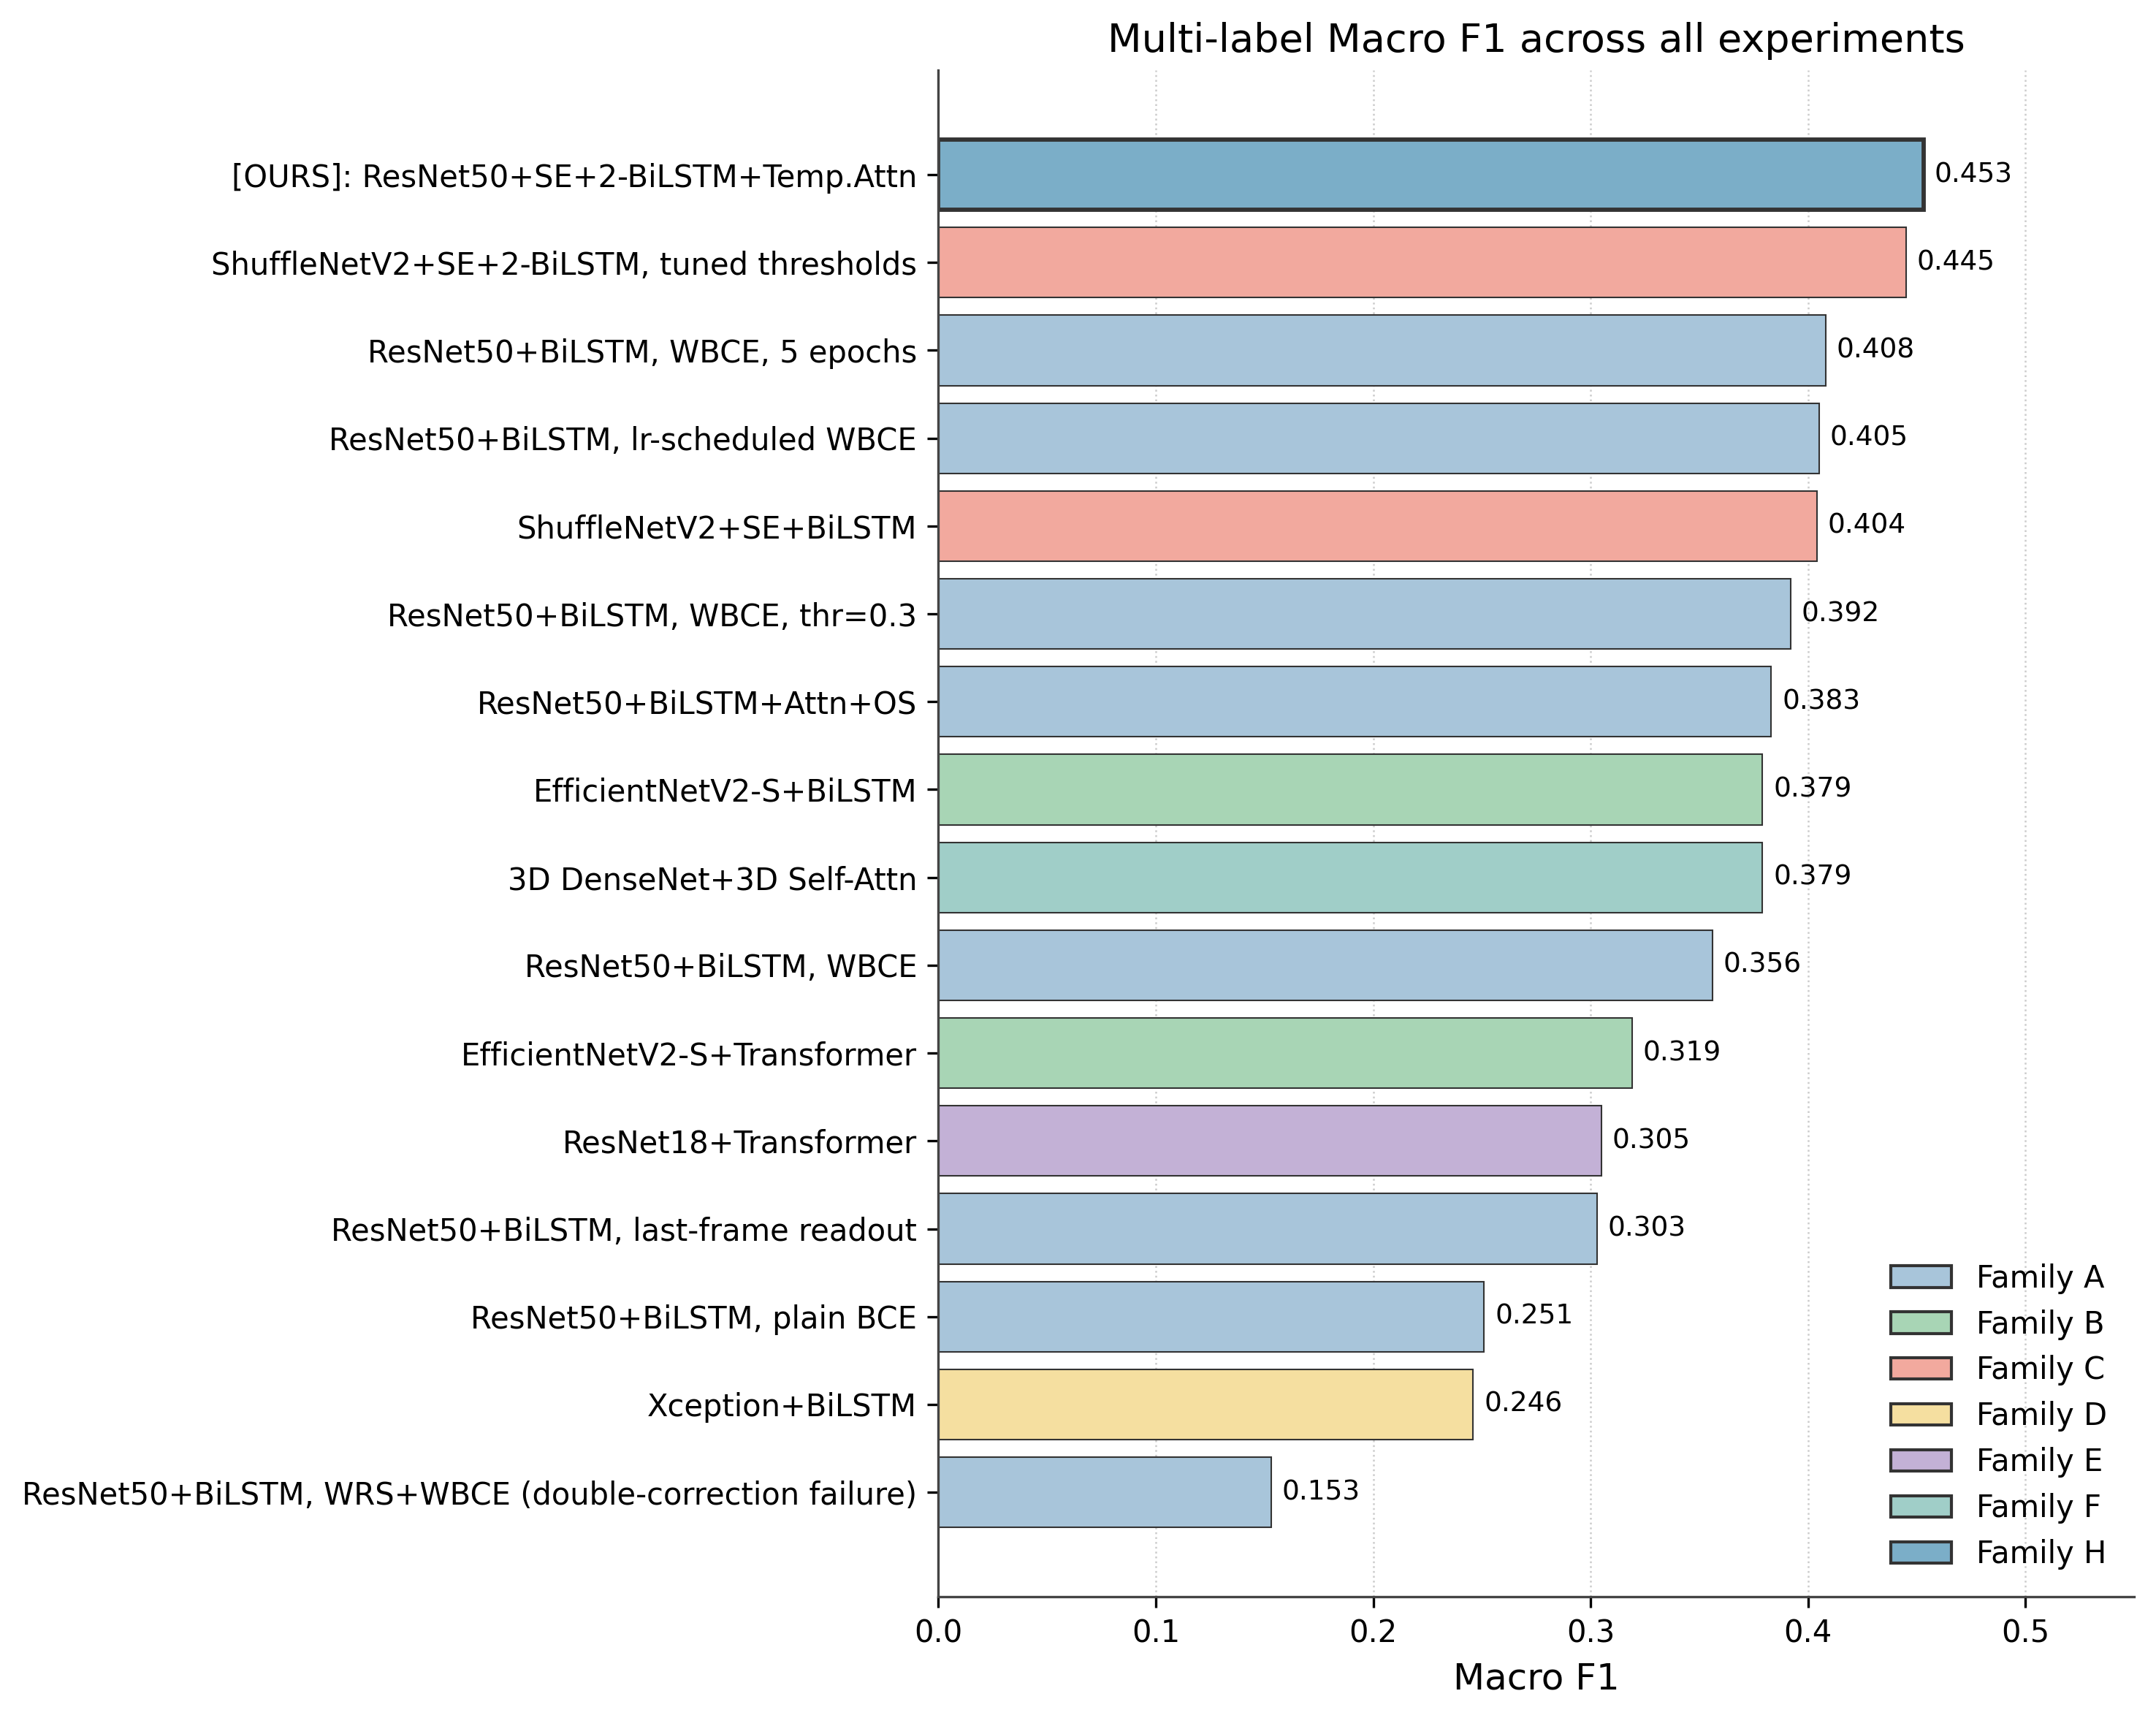
\includegraphics[width=0.92\textwidth]{Figures/import.png}
    \caption{Multi-label Macro F1 for all architectures in
    Table~\ref{tab:fer_multilabel_results}, coloured by backbone
    family. \textbf{[OURS]} is the highest entry.}
    \label{fig:fer_macro_f1_all}
\end{figure}

\subsection{Test Set Performance of [OURS]}\label{sec:results_fer_overall}

\textbf{[OURS]} was evaluated on the $1{,}784$ \ac{DAiSEE} test clips
with per-label thresholds saved at the validation checkpoint
($0.30$ for boredom, $0.10$ for engagement, $0.60$ for confusion,
$0.60$ for frustration) and fixed at test time.

At the overall level, \textbf{[OURS]} reaches Macro F1 $0.453$,
Micro F1 $0.724$, Weighted F1 $0.798$, Samples F1 $0.746$, and
overall label accuracy $0.782$. Weighted F1, Samples F1, and
Micro F1 are dominated by engagement, the most frequent label.
Macro F1 weights all four labels equally and falls below the
others because boredom, confusion, and frustration remain harder
than engagement under imbalance-aware training. Macro F1 is the
primary metric in this thesis because it is the only metric that
does not let engagement dominance hide poor minority-label
performance.

At the per-label level, engagement reaches precision $0.951$,
recall $1.000$, F1 $0.975$, and label accuracy $0.951$. With
$1{,}696$ positive test clips and the lowest tuned threshold
($0.10$), recall is complete; the visual cues for engagement,
alert eyes, stable head pose, and forward-leaning posture, are
also more reliable than the cues for the rare states
\cite{dmello_language_2012,asaju_adaptive_2022,tulsani_realtime_2025}.
Boredom reaches precision $0.239$, recall $0.708$, F1 $0.358$,
and label accuracy $0.462$, an intentional recall-over-precision
trade-off appropriate for an adaptation system that must not miss
disengagement. Confusion reaches precision $0.171$, recall
$0.325$, F1 $0.224$, and label accuracy $0.802$ on $157$ positive
clips, while frustration reaches precision $0.205$, recall
$0.338$, F1 $0.255$, and label accuracy $0.911$ on $80$ positive
clips. Both per-label accuracies above $0.80$ are inflated by the
dominant negative class (``not confused'' prevalence $0.912$,
``not frustrated'' prevalence $0.955$). Both results clear the
relevant benchmark of non-zero recall, which early baselines did
not.

\begin{figure}[H]
    \centering
    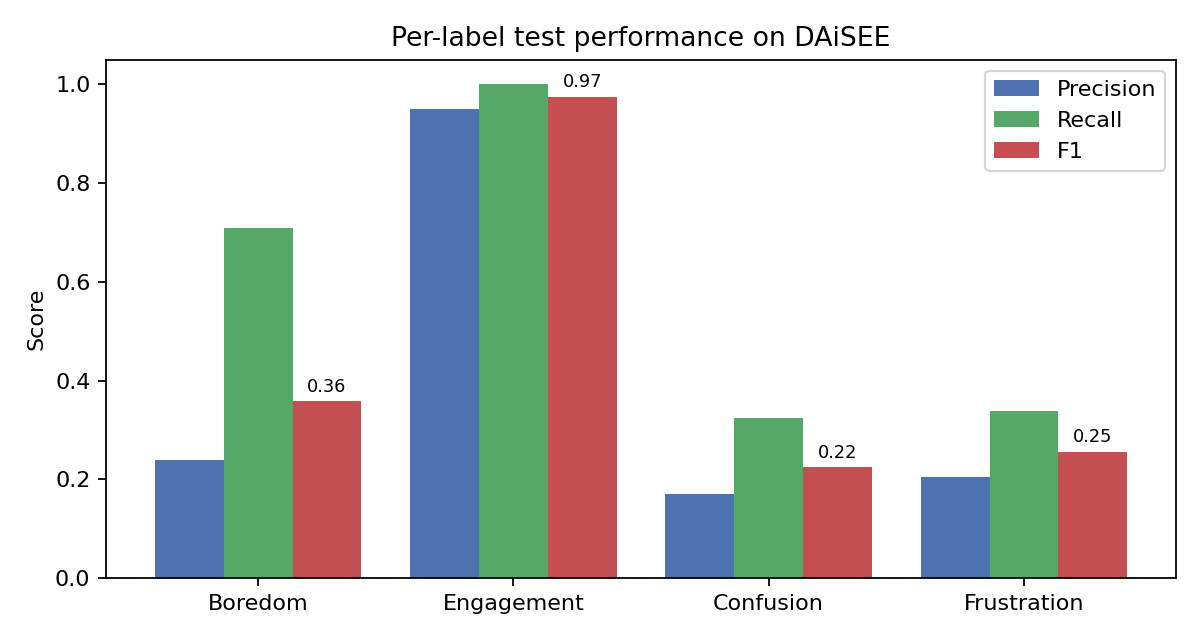
\includegraphics[width=0.92\textwidth]{Figures/fer_per_label_metrics.png}
    \caption{Per-label precision, recall, and F1 of \textbf{[OURS]}
    on the \ac{DAiSEE} test split.}
    \label{fig:fer_per_label_metrics}
\end{figure}

\begin{figure}[H]
    \centering
    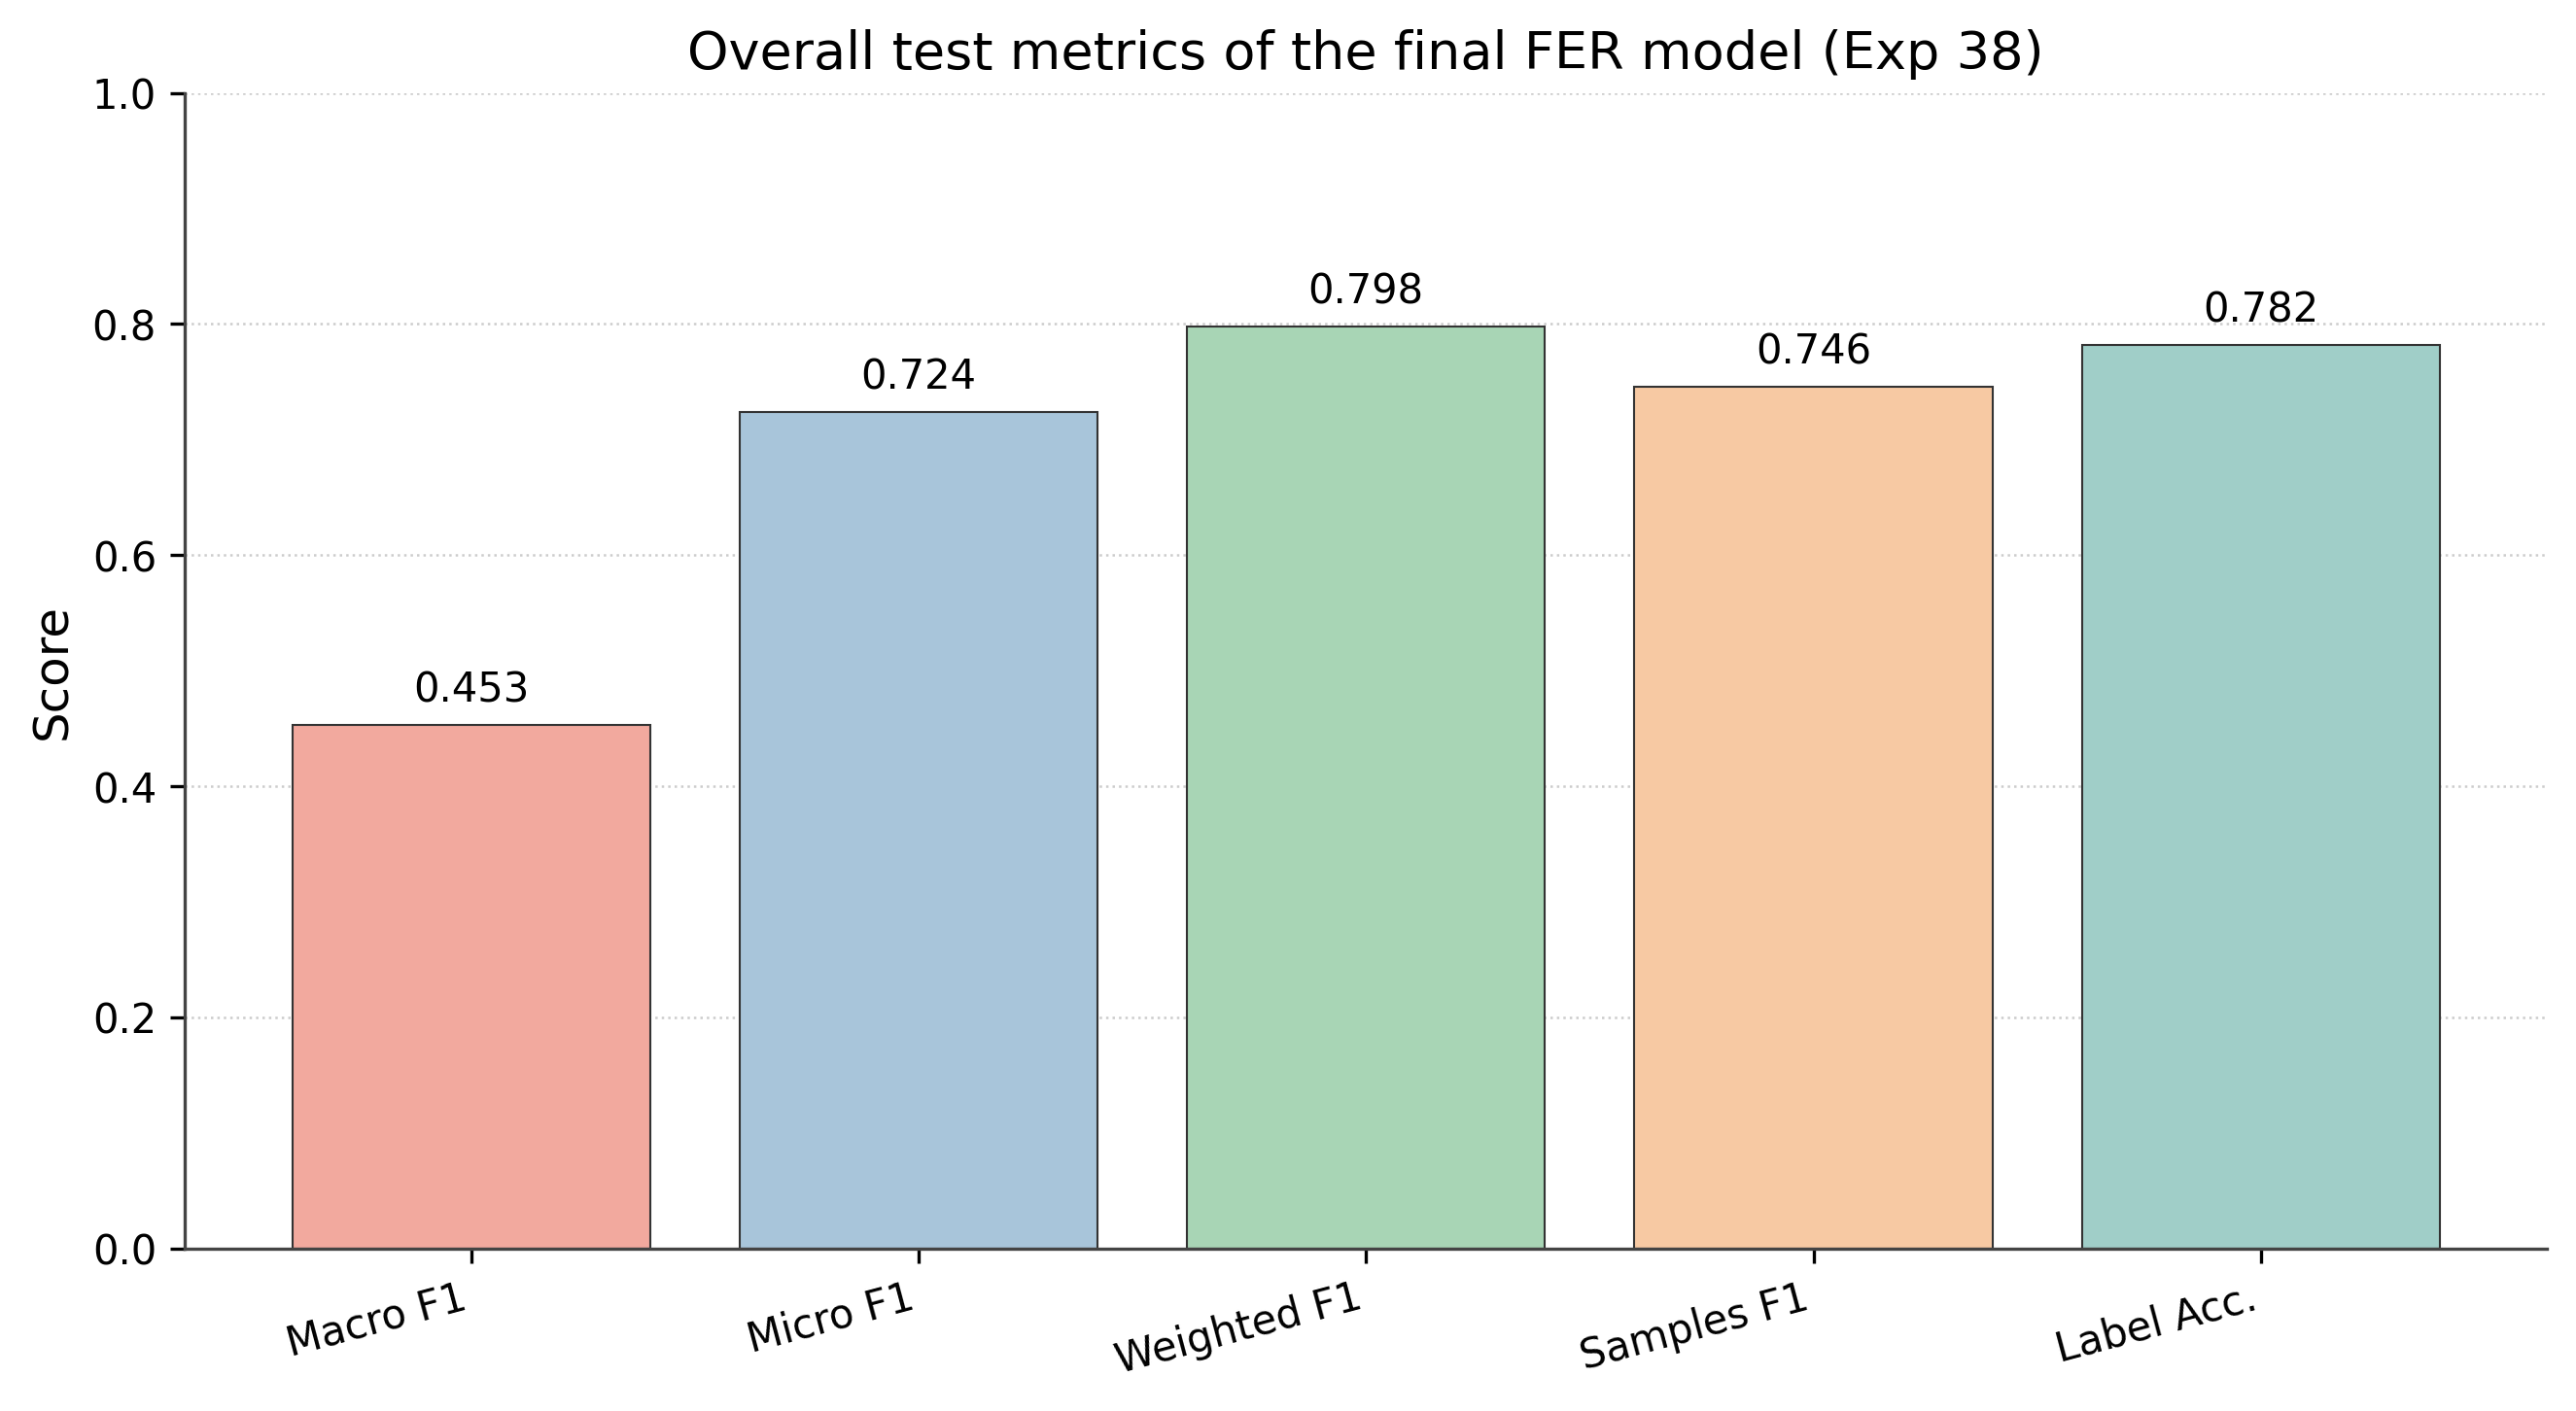
\includegraphics[width=0.85\textwidth]{Figures/fer_overall_metrics_2.png}
    \caption{Overall test metrics of \textbf{[OURS]} on the \ac{DAiSEE}
    test split: Macro F1, Micro F1, Weighted F1, Samples F1, and
    per-label accuracy.}
    \label{fig:fer_overall_metrics}
\end{figure}

\begin{figure}[H]
    \centering
    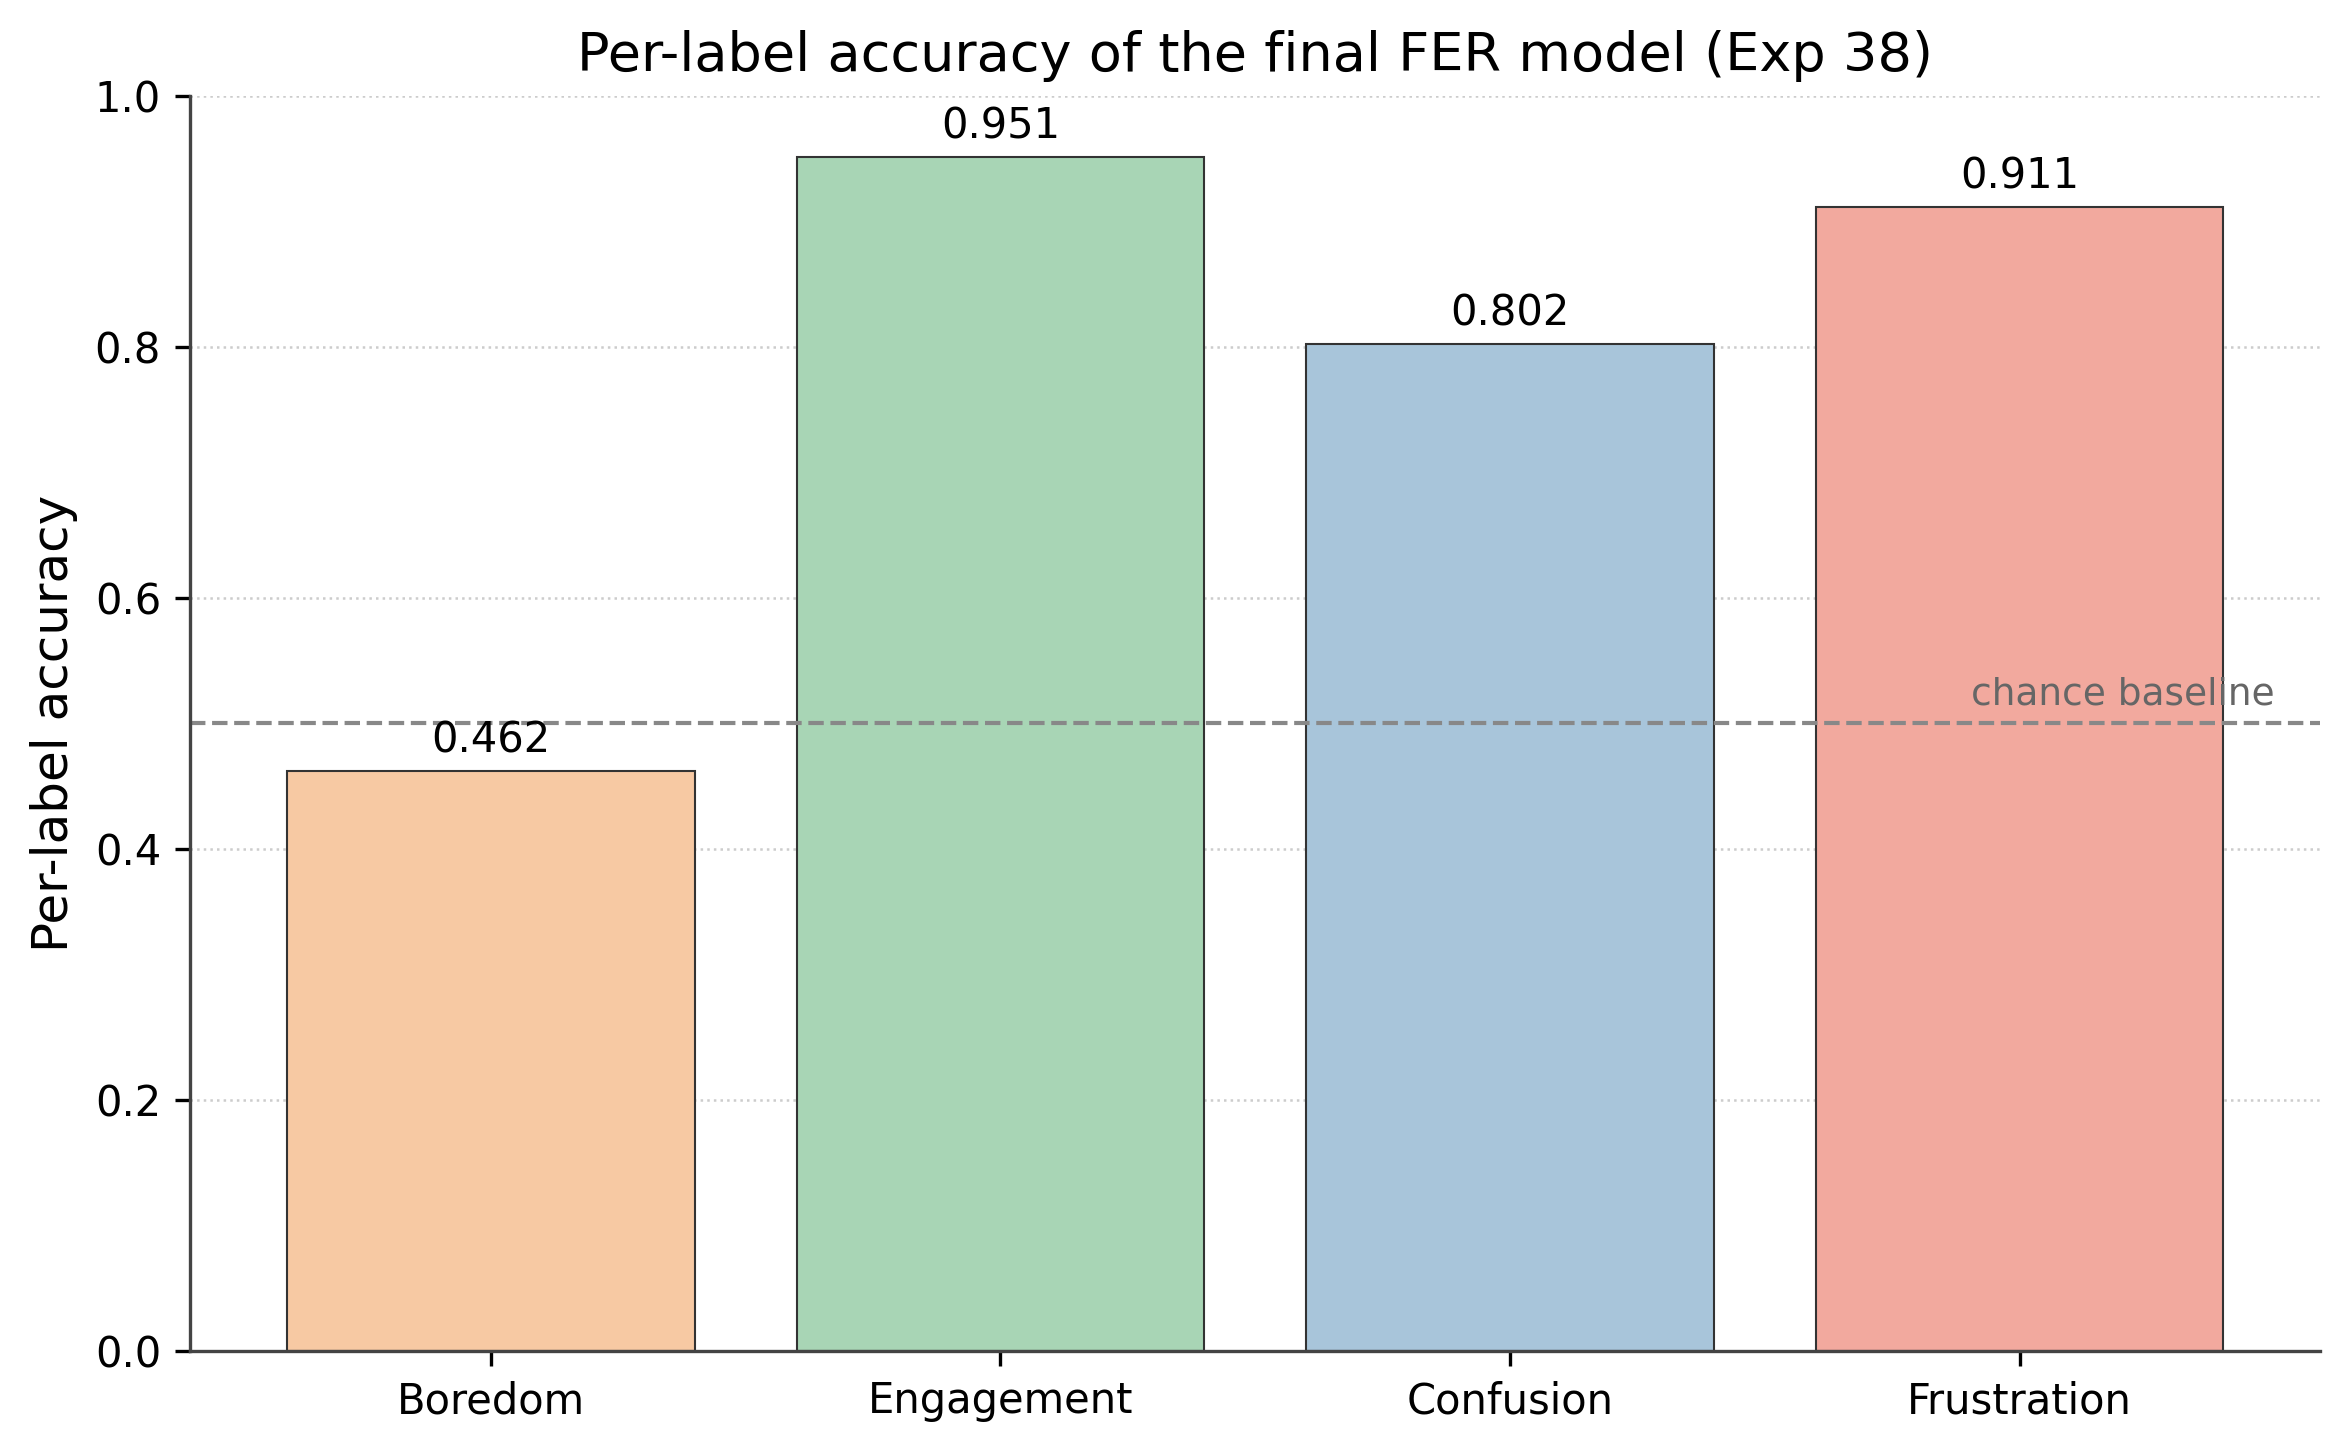
\includegraphics[width=0.85\textwidth]{Figures/fer_per_label_accuracy.png}
    \caption{Per-label accuracy of \textbf{[OURS]}. The dashed line
    at $0.5$ marks the balanced-binary chance baseline.}
    \label{fig:fer_per_label_accuracy}
\end{figure}

\subsection{Training Behaviour}\label{sec:results_fer_training}

Training loss of \textbf{[OURS]} decreases monotonically from
$0.7605$ at epoch $1$ to $0.4938$ at epoch $5$, while validation
Macro F1 peaks at epoch $1$ with $0.5117$ and stays between
$0.4795$ and $0.5000$ thereafter. Validation Micro F1 rises mildly
from $0.6883$ to $0.7348$ and validation Weighted F1 is flat
around $0.76$ across the run. The training loss continues falling
after epoch $1$ while validation Macro F1 has already stopped
improving, the standard signature of mild overfitting reported by
other \ac{CNN}-plus-recurrent \ac{DAiSEE} pipelines at small batch sizes
\cite{abedi_improving_2021,mehta_three-dimensional_2022,shiri_detection_2024}.
Early stopping selects the epoch-$1$ checkpoint because the
ResNet50 backbone, initialised from ImageNet and fine-tuned at a
small learning rate, has most of the visual representation needed
for academic affect already in place at the start of training
(Figure~\ref{fig:fer_training_curves}).

\begin{figure}[H]
    \centering
    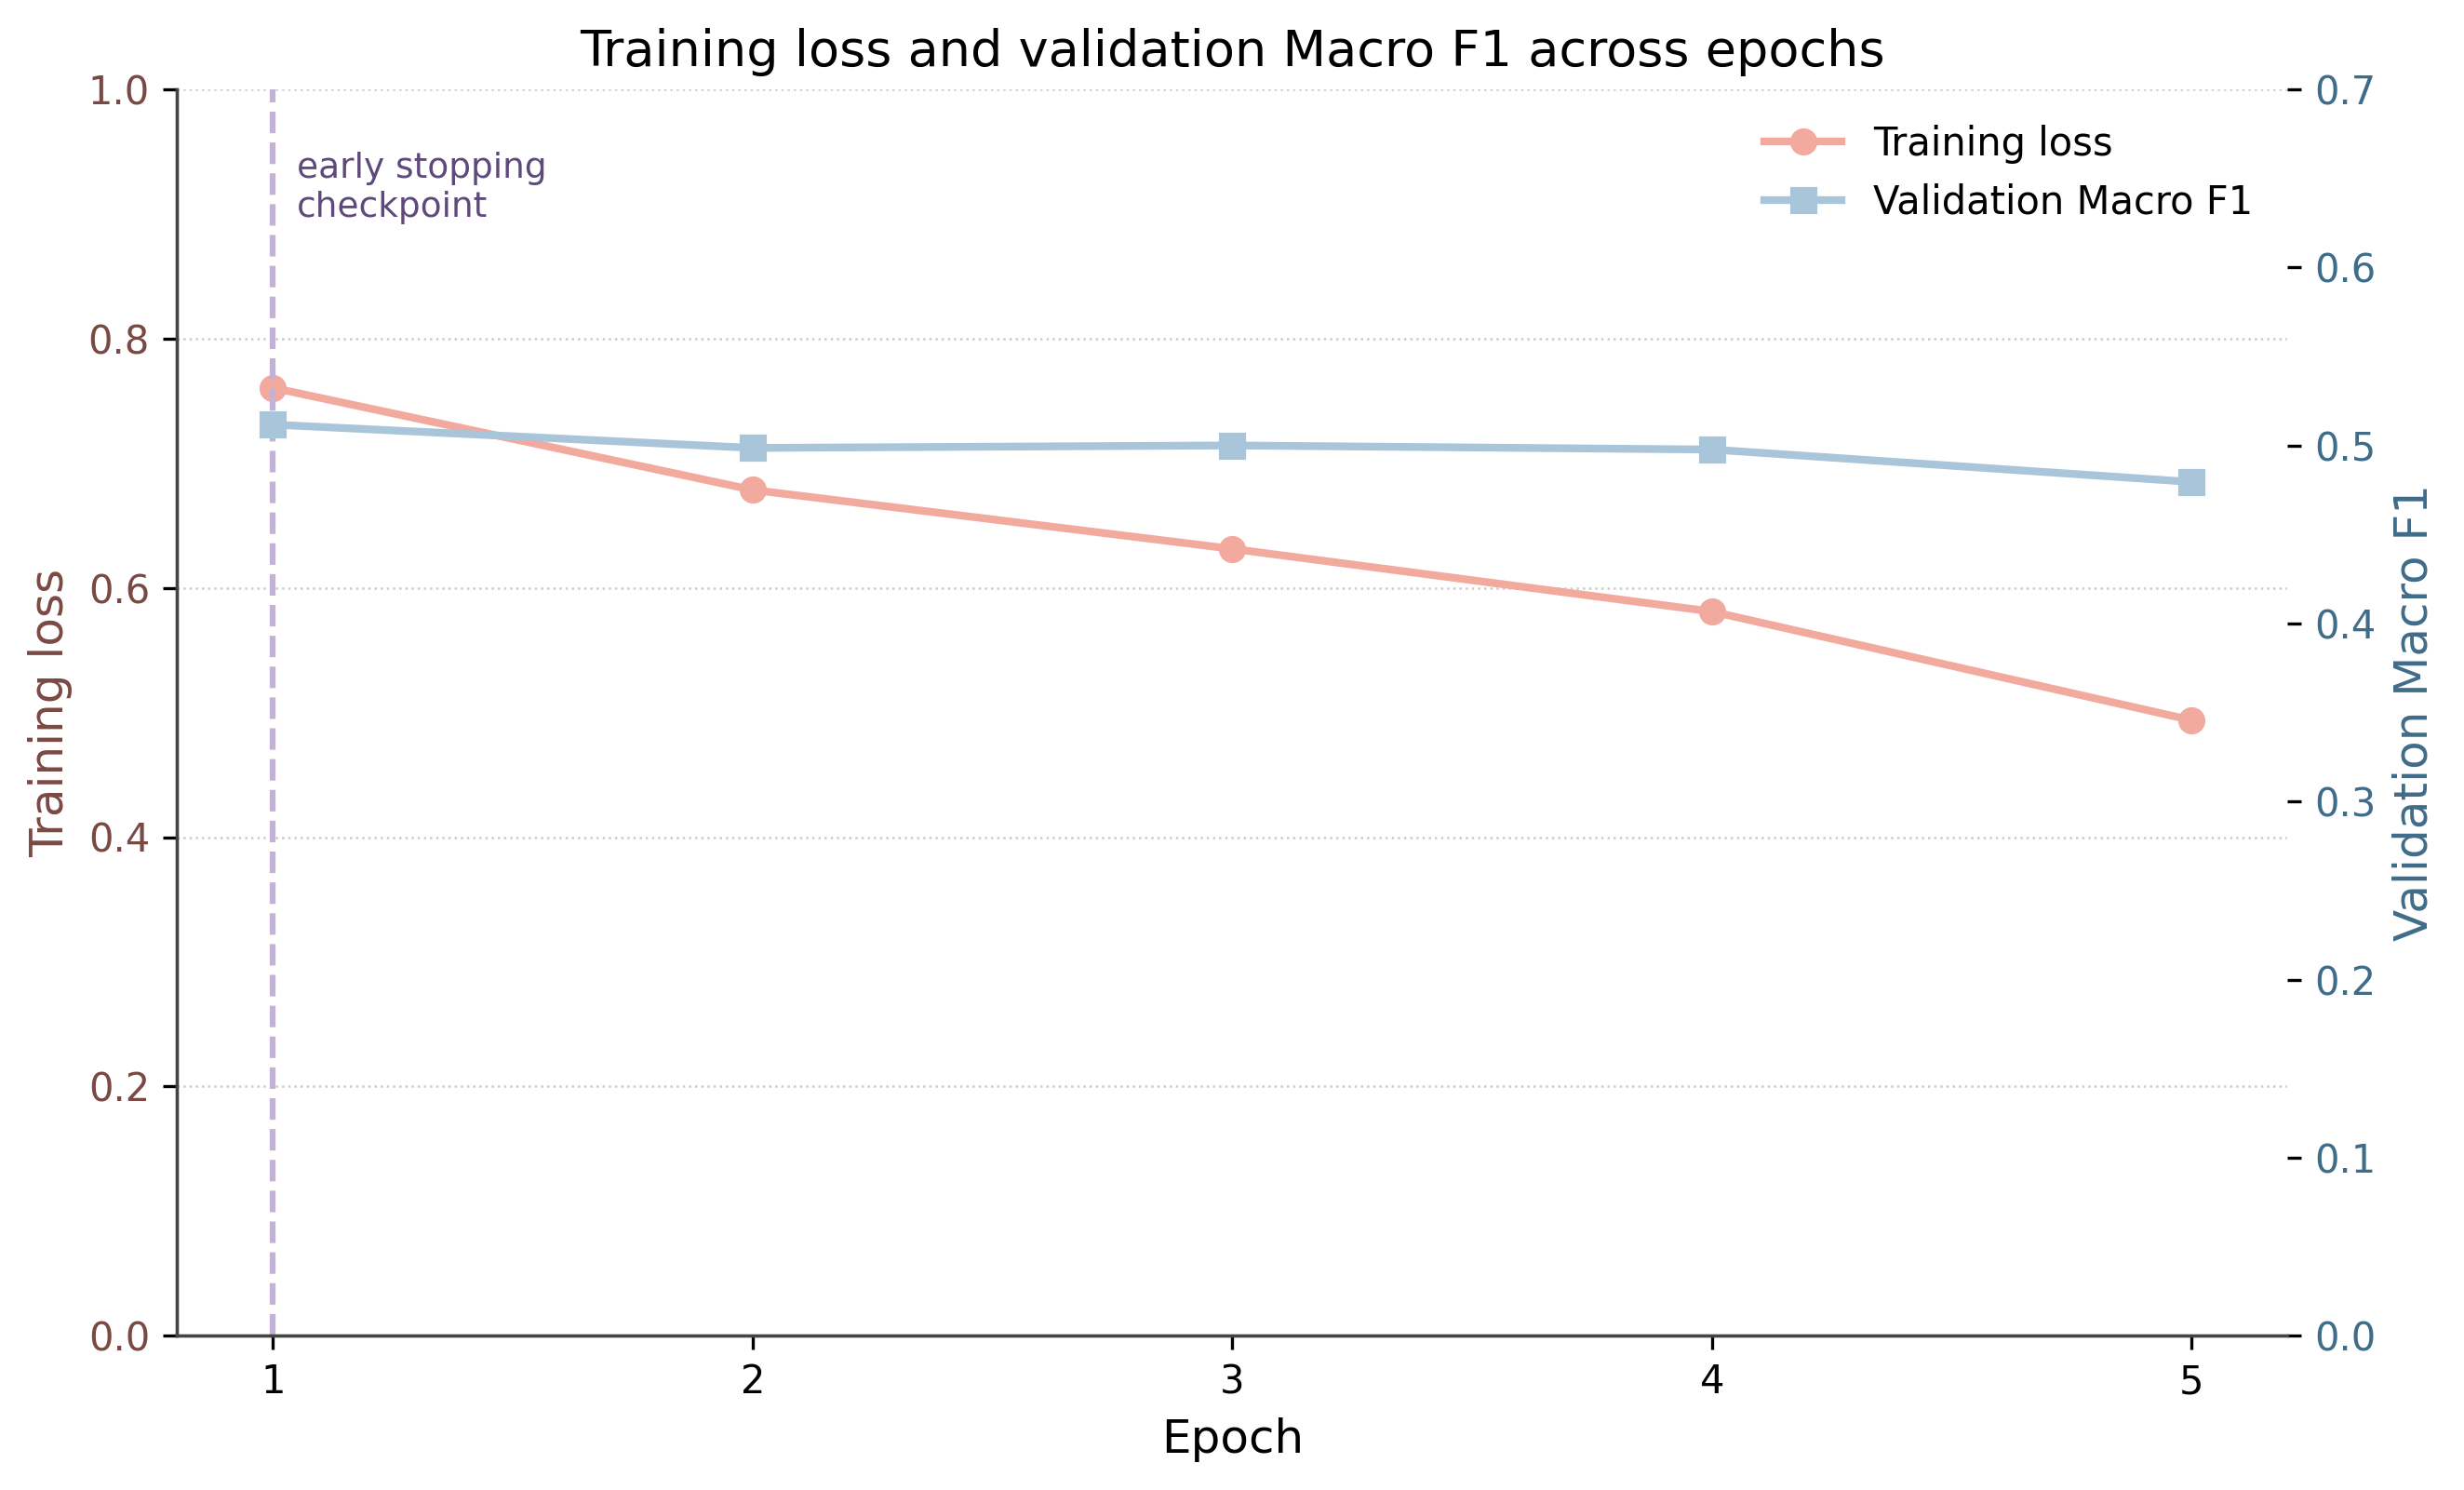
\includegraphics[width=0.88\textwidth]{Figures/fer_training_curves_2.png}
    \caption{Training loss and validation Macro F1 across epochs
    for \textbf{[OURS]}. The dashed line at epoch $1$ marks the
    early-stopping checkpoint.}
    \label{fig:fer_training_curves}
\end{figure}

\subsection{Literature Context}\label{sec:results_fer_literature}

Most prior \ac{DAiSEE} work simplifies the task to a single-label
four-class engagement problem and evaluates under undisclosed
preprocessing. Reported metrics therefore reflect heterogeneous
evaluation environments.
Table~\ref{tab:fer_lit_compare} lists the prior work and the
relationship each source has to this thesis. The Relationship
column uses \textit{Inspired by} when only a backbone or
component was borrowed, \textit{Reproduced under our pipeline}
when the architecture was retrained from scratch under the
standardised setup, and \textit{Component borrowed} for a
temporal or attention module re-used in modified form.
% Excluded from this table:
%   - Komaravalli & B (2023), Scalable Computing 24(4), 957-970:
%     evaluates on a customized \ac{DAiSEE} subset, not the standard
%     train/val/test split, so not directly comparable.
%   - Rezaee et al. (2024), Journal on Artificial Intelligence 6(1),
%     85-103: evaluates engagement-only (single label, 4-level
%     ordinal), so not comparable to a 4-state multilabel system.
\begin{table}[H]
\centering
\footnotesize
\caption{Prior \ac{FER} work on \ac{DAiSEE} and its relationship to this thesis.}
\label{tab:fer_lit_compare}
\setlength{\tabcolsep}{4pt}
\begin{threeparttable}
\begin{tabular}{p{3.0cm} p{2.2cm} p{2.4cm} p{1.4cm} c c p{2.6cm}}
\toprule
\textbf{Work} & \textbf{Backbone} & \textbf{Temporal / Attention} &
\textbf{Labels} & \textbf{Accuracy (\%)} & \textbf{Macro F1}$^{\ddagger}$ &
\textbf{Relationship} \\
\midrule
Gupta et al.\ \cite{gupta_daisee_2016}            & C3D / I3D         & 3D \ac{CNN}              & 4-state ML  & 57.9$^{\dagger}$ & ---   & Dataset paper, used as baseline \\
Abedi and Khan \cite{abedi_improving_2021}        & ResNet            & \ac{TCN}                 & Eng.\ only  & 63.9             & ---   & Inspired by, component borrowed (\ac{TCN} head) \\
Mehta et al.\ \cite{mehta_three-dimensional_2022} & 3D DenseNet       & 3D self-attention   & Eng.\ only  & 63.6             & ---   & Reproduced under our pipeline \\
Shiri et al.\ \cite{shiri_detection_2024}         & EfficientNetV2-L  & RNN                 & Eng.\ only  & 62.11            & ---   & Backbone borrowed, downsized to V2-S \\
\midrule
\textbf{[OURS]} & \textbf{ResNet50 + \ac{SE}} & \textbf{2-\ac{BiLSTM} + temp.\ attn.} & \textbf{4-state ML} & \textbf{78.2} & \textbf{0.453} & \textbf{Proposed system} \\
\bottomrule
\end{tabular}
\begin{tablenotes}
\footnotesize
\item[$\dagger$] The 57.9\% for Gupta et al.\ is the average of per-class top-1 accuracy across four affective states (Boredom 53.7\%, Engagement 57.9\%, Confusion 72.3\%, Frustration 73.5\%) for their best model (LRCN); a single overall accuracy is not reported.
\item[$\ddagger$] Macro F1 is not reported by any prior work in this table; these works use single-label multiclass accuracy on engagement-only or per-class top-1 accuracy, and Macro F1 across all four affective states cannot be inferred from their reported numbers.
\end{tablenotes}
\end{threeparttable}
\end{table}

\begin{table}[H]
\centering
\footnotesize
\caption{Extended \ac{DAiSEE} accuracy comparisons from works using non-standard or engagement-only evaluation protocols (reproduced from cited sources).}
\label{tab:fer_extended_compare}
\setlength{\tabcolsep}{6pt}
\begin{threeparttable}
\begin{tabular}{p{4.2cm} c p{3.2cm}}
\toprule
\textbf{Method} & \textbf{Accuracy (\%)} & \textbf{Source} \\
\midrule
\multicolumn{3}{l}{\textit{Komaravalli \& B \cite{komaravalli_detecting_2023} --- customized \ac{DAiSEE} subset$^{\S}$}} \\
Video-level InceptionNet              & 46.40 & \cite{komaravalli_detecting_2023} \\
Frame-level InceptionNet              & 47.10 & \cite{komaravalli_detecting_2023} \\
C3D feature extraction                & 48.60 & \cite{komaravalli_detecting_2023} \\
I3D                                   & 52.35 & \cite{komaravalli_detecting_2023} \\
ResNet + \ac{TCN} with weighted loss       & 53.70 & \cite{komaravalli_detecting_2023} \\
C3D fine tuning                       & 56.10 & \cite{komaravalli_detecting_2023} \\
C3D (focal loss)                      & 56.20 & \cite{komaravalli_detecting_2023} \\
LRCN                                  & 57.90 & \cite{komaravalli_detecting_2023} \\
DFSTN                                 & 58.84 & \cite{komaravalli_detecting_2023} \\
C3D + \ac{TCN}                             & 59.97 & \cite{komaravalli_detecting_2023} \\
DERN                                  & 60.00 & \cite{komaravalli_detecting_2023} \\
ResNet + \ac{LSTM}                         & 61.15 & \cite{komaravalli_detecting_2023} \\
ResNet + \ac{TCN}                          & 63.90 & \cite{komaravalli_detecting_2023} \\
3D DenseAttNet                        & 63.59 & \cite{komaravalli_detecting_2023} \\
\textbf{Ours (Komaravalli \& B)}      & \textbf{64.00} & \cite{komaravalli_detecting_2023} \\
\midrule
\multicolumn{3}{l}{\textit{Rezaee et al.\ \cite{rezaee_detection_2024} --- engagement-only, single-label \ac{DAiSEE}$^{\P}$}} \\
InceptionNet                              & 46.40 & \cite{rezaee_detection_2024} \\
C3D fine-tuning                           & 56.10 & \cite{rezaee_detection_2024} \\
LRCN                                      & 57.90 & \cite{rezaee_detection_2024} \\
I3D                                       & 52.35 & \cite{rezaee_detection_2024} \\
C3D (FL)                                  & 56.20 & \cite{rezaee_detection_2024} \\
ResNet+\ac{TCN}                                & 53.60 & \cite{rezaee_detection_2024} \\
DFSTN                                     & 58.84 & \cite{rezaee_detection_2024} \\
DERN                                      & 60.00 & \cite{rezaee_detection_2024} \\
Neural Turing Machine                     & 61.30 & \cite{rezaee_detection_2024} \\
ResNet+\ac{TCN} with weighted loss             & 53.70 & \cite{rezaee_detection_2024} \\
C3D+\ac{TCN}                                   & 59.97 & \cite{rezaee_detection_2024} \\
ResNet+\ac{LSTM}                               & 61.15 & \cite{rezaee_detection_2024} \\
ResNet+\ac{TCN}                                & 63.90 & \cite{rezaee_detection_2024} \\
DenseAttNet                               & 63.59 & \cite{rezaee_detection_2024} \\
EfficientNetV2-L+\ac{GRU}                      & 61.45 & \cite{rezaee_detection_2024} \\
EfficientNetV2-L+Bi-\ac{GRU}                   & 61.56 & \cite{rezaee_detection_2024} \\
\textbf{EfficientNetV2-L+\ac{LSTM} (proposed)} & \textbf{62.11} & \cite{rezaee_detection_2024} \\
EfficientNetV2-L+Bi-\ac{LSTM}                  & 61.67 & \cite{rezaee_detection_2024} \\
\bottomrule
\end{tabular}
\begin{tablenotes}
\footnotesize
\item[$\S$] Komaravalli \& B trained and evaluated on a customized filtered subset of \ac{DAiSEE}, not the standard train/val/test split. Results are not directly comparable to systems using the standard protocol.
\item[$\P$] Rezaee et al.\ evaluate on engagement-only (single label, 4-level ordinal) rather than all four affective states. Accuracy figures reflect engagement classification only and are not comparable to 4-state multilabel systems.
\end{tablenotes}
\end{threeparttable}
\end{table}

\noindent Reported values reflect each paper's original
evaluation environment. Direct numerical comparison with
\textbf{[OURS]} is not appropriate.

The numbers in Table~\ref{tab:fer_lit_compare} cannot be ranked
against each other or against \textbf{[OURS]}: each source uses
its own preprocessing, splits, and label definitions, and Su et
al.'s comparison table aggregates many methods across
heterogeneous setups, so it cannot serve as a unified benchmark.
Two characteristics nonetheless distinguish \textbf{[OURS]}:
it is the only configuration evaluated in this thesis that
performs four-state multi-label classification on \ac{DAiSEE} under a
single standardised pipeline, and its architecture is based on
widely available deep-learning components that can be reproduced
using commonly accessible GPU hardware.

\subsection{Discussion}\label{sec:results_fer_discussion}

\noindent\textbf{1. Accuracy is misleading on \ac{DAiSEE}.}
The \ac{HOG}+\ac{LBP}+\ac{SVM} baseline reaches $0.750$ accuracy by predicting
engagement on almost every clip, with zero F1 on the three
minority labels. The strongest single-label deep model reaches
$0.702$ accuracy with minority F1 below $0.13$. \textbf{[OURS]}
reports per-label accuracy of $0.911$ on frustration despite F1
of $0.255$ because $95.5\%$ of test clips are not frustrated.
Macro F1 is the only metric that does not hide this collapse.
Figure~\ref{fig:fer_svm_vs_final} makes the same point visually.

\begin{figure}[H]
    \centering
    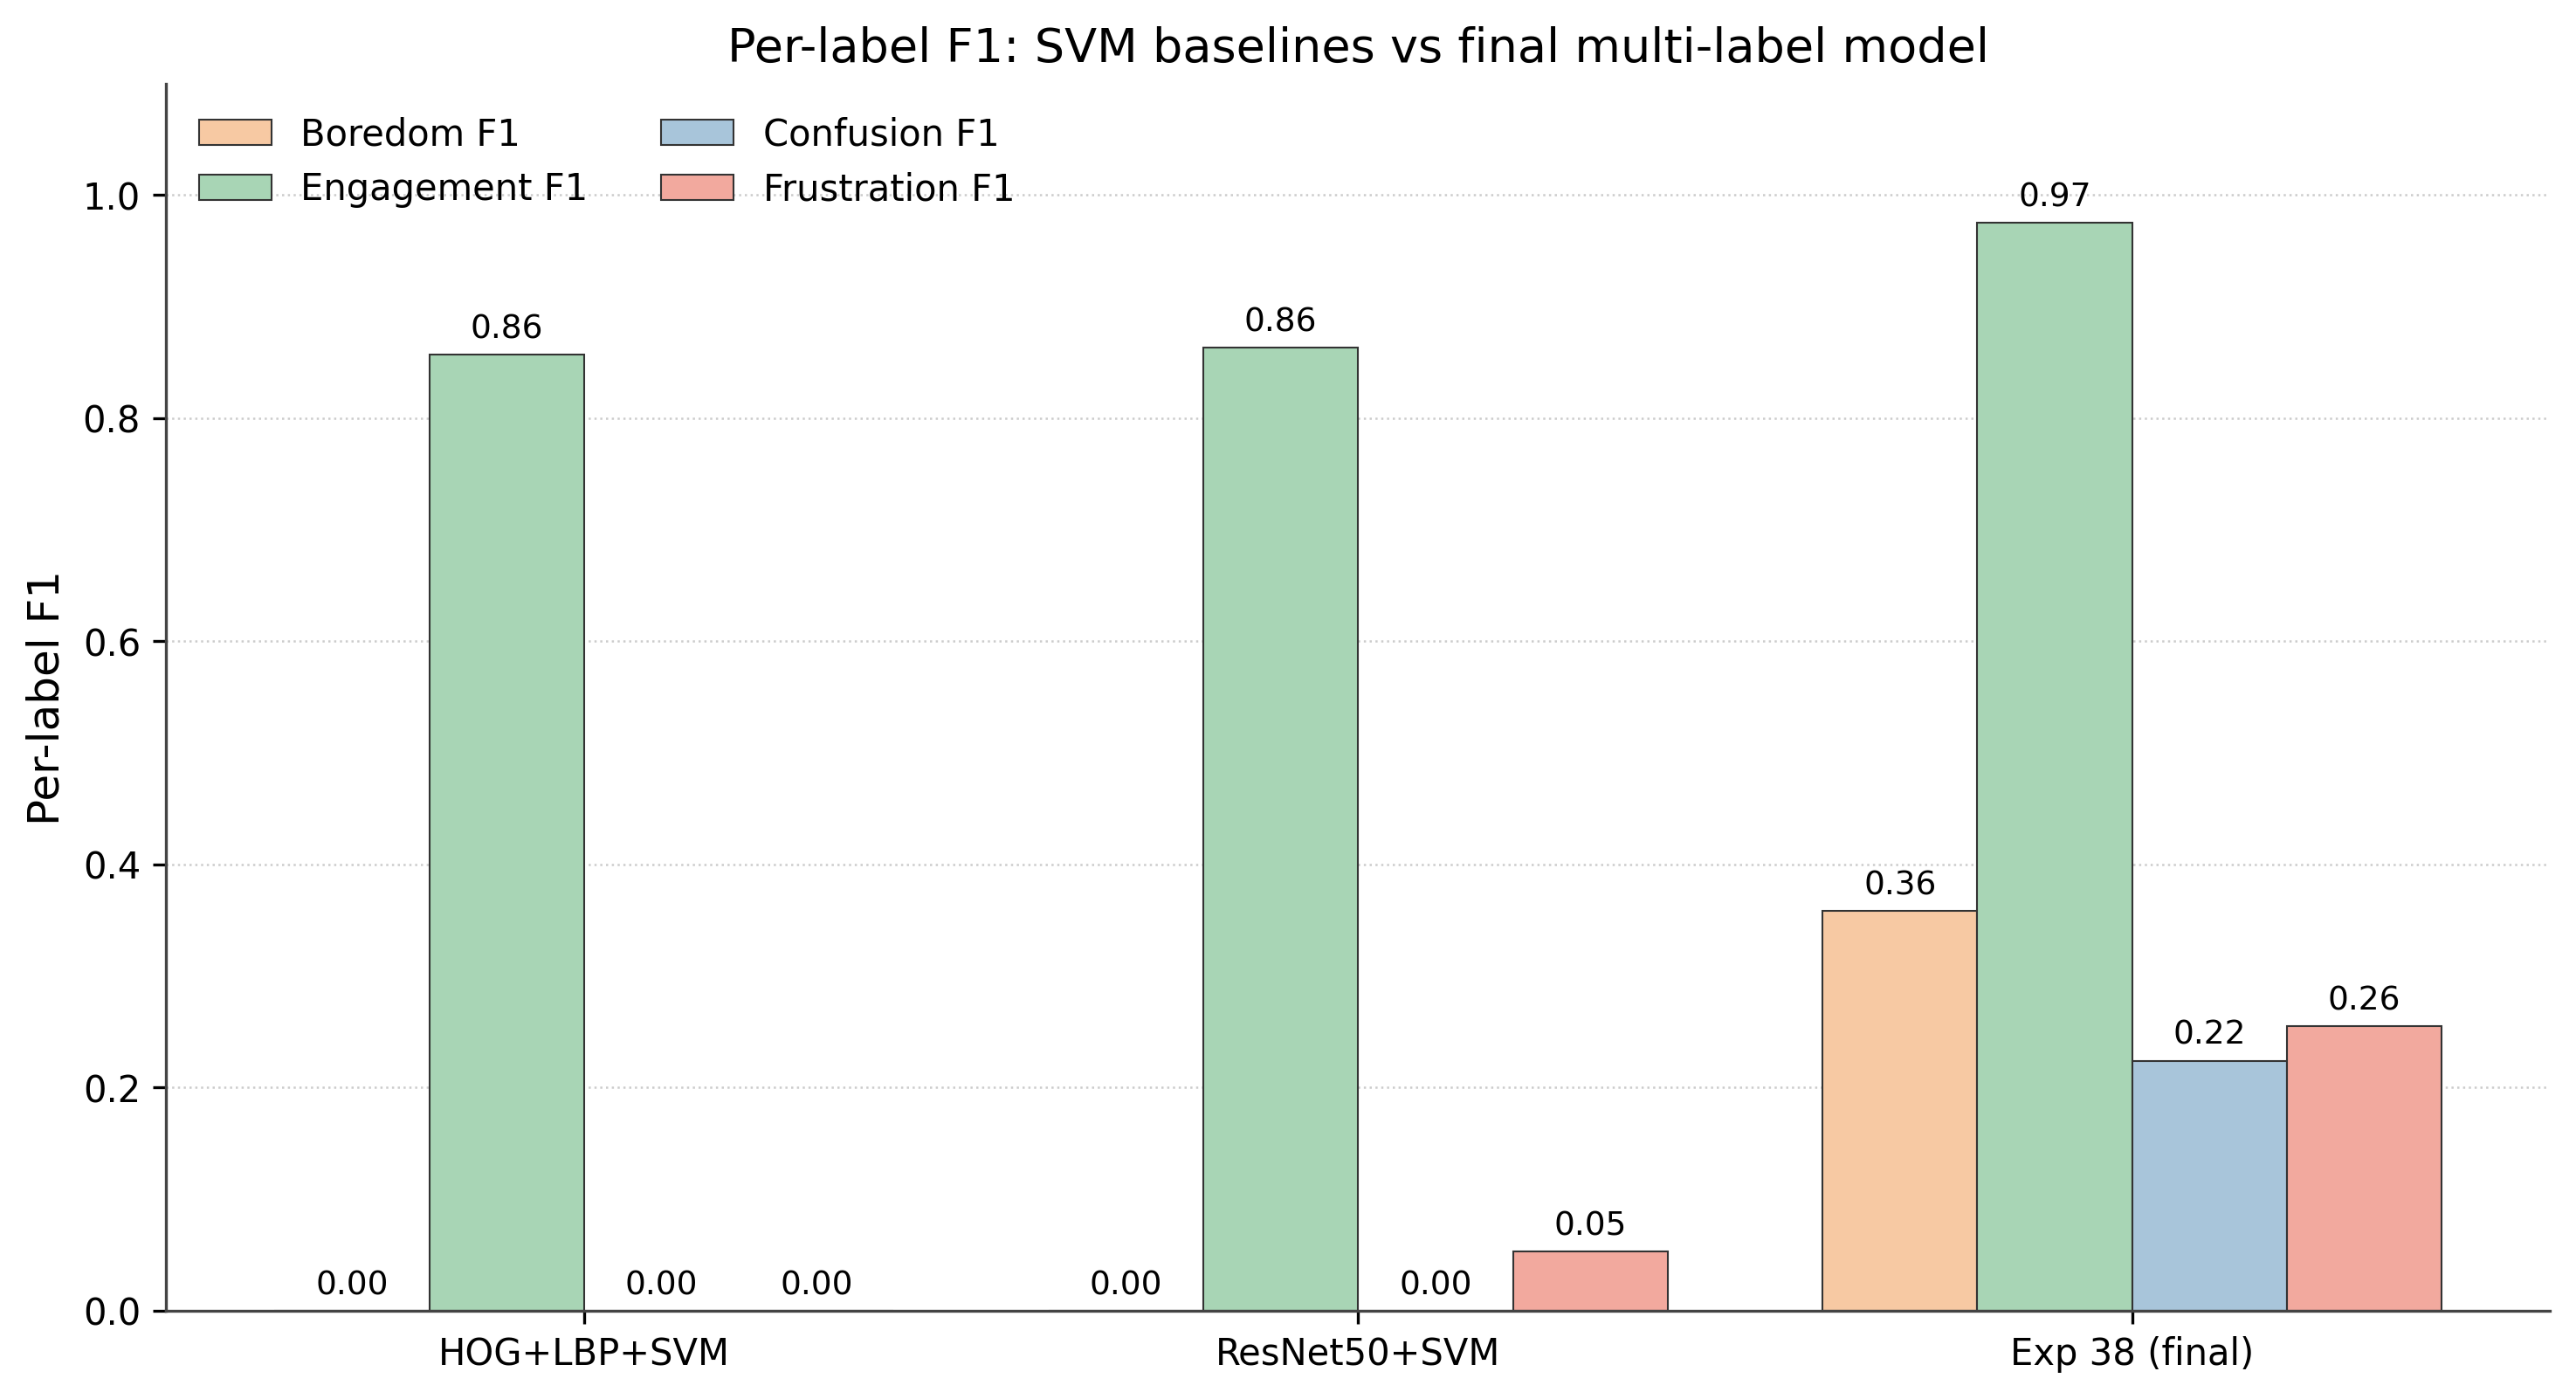
\includegraphics[width=0.92\textwidth]{Figures/fer_svm_vs_final.png}
    \caption{Per-label F1 of the \ac{SVM} baselines and
    \textbf{[OURS]}. The \ac{SVM} baselines have non-zero F1 only on
    engagement.}
    \label{fig:fer_svm_vs_final}
\end{figure}

\noindent\textbf{2. Imbalance must be addressed at every level.}
Plain \ac{BCE} collapses to Macro F1 $0.251$. Loss-level correction
alone, weighted \ac{BCE}, reaches $0.408$. Stacking a
WeightedRandomSampler on top of weighted \ac{BCE} applies two
corrections to the same imbalance and over-corrects: engagement
F1 falls to zero and Macro F1 drops to $0.153$. The combination
used by \textbf{[OURS]}, mild fixed-multiplier oversampling with
clipped positive-class weights and per-label tuned thresholds,
reaches $0.453$. Figure~\ref{fig:fer_familyA_progression} traces
this progression. No single intervention is sufficient; the three
levels must be calibrated jointly.

\begin{figure}[H]
    \centering
    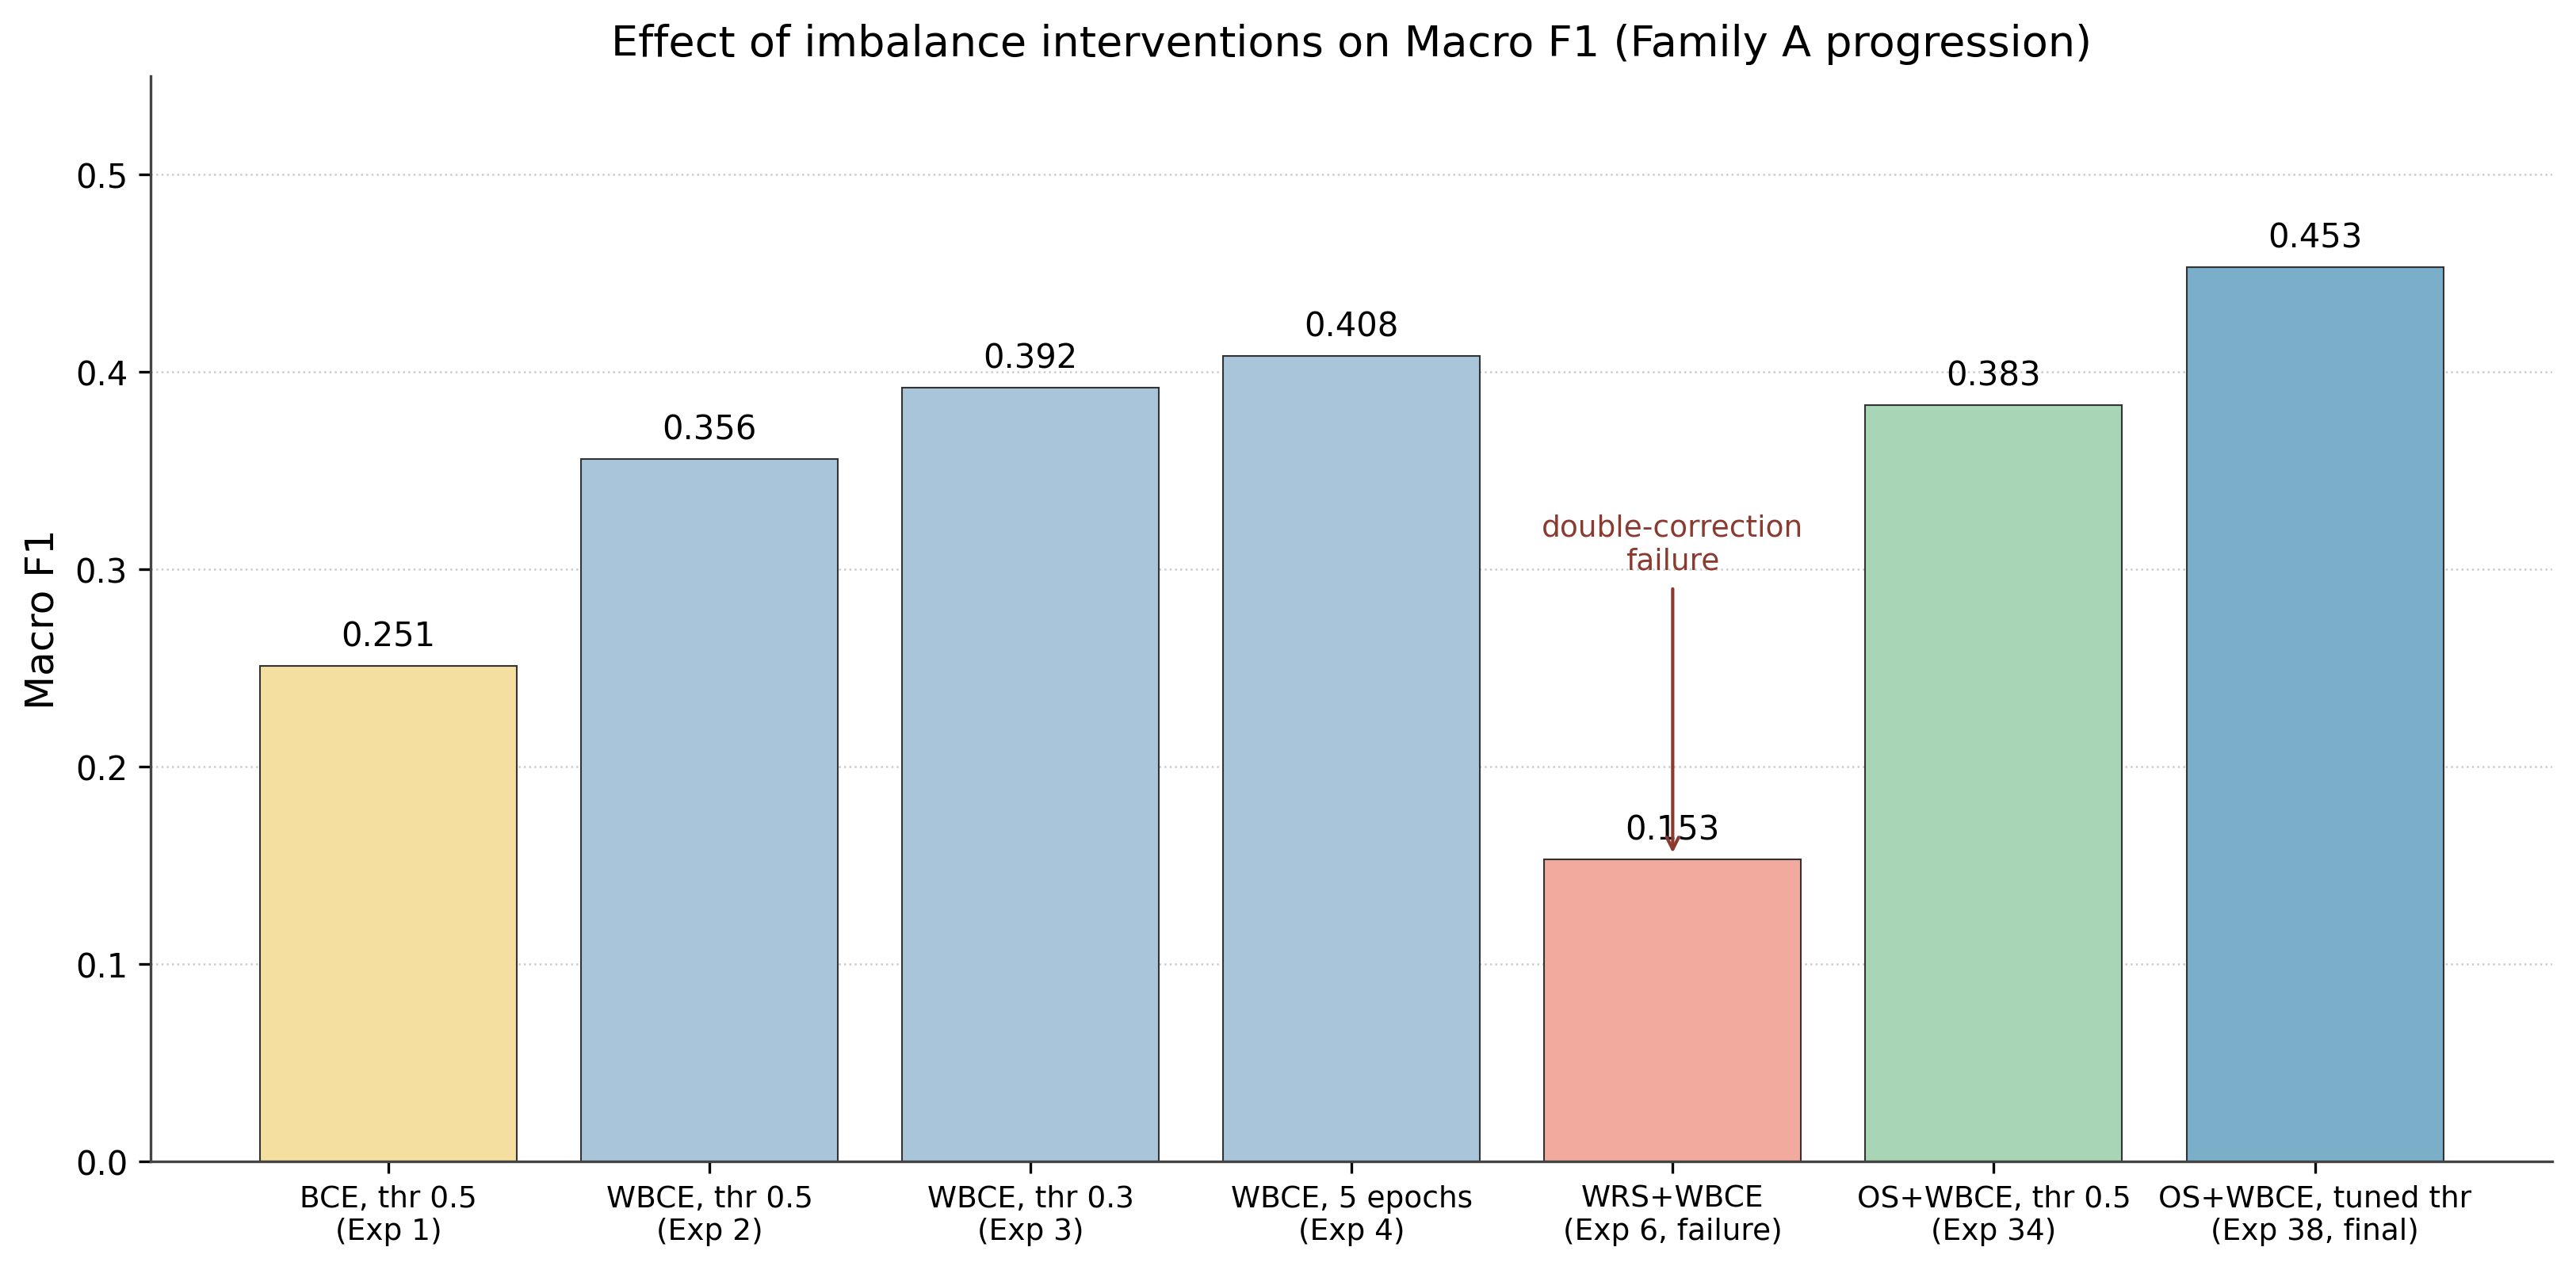
\includegraphics[width=0.92\textwidth]{Figures/fer_familyA_progression.png}
    \caption{Macro F1 progression through the ResNet50+\ac{BiLSTM}
    ablation. The WRS+WBCE double-correction failure is highlighted
    in coral; \textbf{[OURS]} is the highest entry.}
    \label{fig:fer_familyA_progression}
\end{figure}

\noindent\textbf{3. Heavier or more recent backbones do not help at
this scale.} EfficientNetV2-S \cite{shiri_detection_2024} reaches
Macro F1 $0.379$, below the lightweight ShuffleNetV2+\ac{SE}
\cite{aly_revolutionizing_2025} at $0.404$. The 3D
DenseNet with self-attention \cite{mehta_three-dimensional_2022},
the heaviest model tested, also reaches $0.379$. With only
$5{,}358$ \ac{DAiSEE} training clips, backbone scaling does not behave
as on ImageNet, a pattern consistent with recent educational \ac{FER}
reviews
\cite{lek_academic_2023,vistorte_integrating_2024,florestiyanto_emotion_2024}.

\noindent\textbf{4. Per-label threshold tuning is the most
cost-effective intervention.} Moving a fixed threshold from $0.5$
to $0.3$ on the same network raises Macro F1 from $0.356$ to
$0.392$. Per-label tuned thresholds reach $0.445$ and $0.453$, the
two highest entries in Table~\ref{tab:fer_multilabel_results}, and
require no retraining once the validation pass is complete.

\noindent\textbf{5. Confusion and frustration remain hard.}
Confusion F1 $0.224$ on $157$ positive clips and frustration F1
$0.255$ on $80$ positive clips are the principal limitations of
\textbf{[OURS]}. Both labels are rare, ambiguous, and often
suppressed by learners facing a webcam. The per-label thresholds
favour recall, which is the appropriate operating point for the
adaptation module but caps precision. Pushing these two labels
further would require additional modalities (audio, posture,
log-stream signals) or a larger affective video corpus.

\subsection{Summary}\label{sec:results_fer_summary}

\textbf{[OURS]} achieves the following on the \ac{DAiSEE} test set:
\begin{itemize}
    \item \textbf{Architecture:} ResNet50 + \ac{SE} block + two-layer
    \ac{BiLSTM} + temporal attention, trained on 24-frame clips.
    \item \textbf{Training:} Weighted \ac{BCE} loss with fixed-multiplier
    oversampling (OS-CSV) and per-label thresholds tuned on the
    validation split.
    \item \textbf{Macro F1:} $0.453$. \textbf{Weighted F1:} $0.798$.
    \textbf{Micro F1:} $0.724$. \textbf{Samples F1:} $0.746$.
    \item \textbf{Per-label F1:} Boredom $0.358$ $|$ Engagement
    $0.975$ $|$ Confusion $0.224$ $|$ Frustration $0.255$.
    \item \textbf{Principal limitation:} Precision-recall trade-off
    on confusion and frustration, the two rarest and visually most
    ambiguous labels.
    \item \textbf{Distinction:} The only configuration combining
    four-state multi-label \ac{DAiSEE} classification with calibrated,
    reproducible, deployment-ready thresholds under a single
    standardised pipeline.
\end{itemize}

The four-dimensional emotion vector produced by \textbf{[OURS]},
one binary label per affective state per clip, serves as the
affect input to the reinforcement-learning adaptation module
described in the following section.

% =====================================================================
% =====================================================================
% PART II - ADAPTATION MODULE RESULTS AND DISCUSSION
% =====================================================================

\section{Adaptation Module Results and Discussion}\label{sec:results_adapt_part}

\subsection{Experimental Overview}\label{sec:results_adapt_overview}

Section~\ref{sec:results_adapt_part} reports the evaluation of
the adaptation module specified in Chapter~4. Two student
populations are used: a single canonical learner
(Configuration~A) that exposes overfitting and a heterogeneous
mixed population (Configuration~B) that mirrors the deployment
setting. The trained \ac{DQN} policy is compared with a rule-based
expert tutor and a uniform random policy under identical
evaluation episodes and ten independent seeds; a twenty-seed
confirmation run was performed for Configuration~B.
Section~\ref{sec:results_adapt_comparison} reports the headline
comparison, Section~\ref{sec:results_adapt_robustness} reports
robustness and generalisation,
Section~\ref{sec:results_adapt_literature} positions the system
against prior work, Section~\ref{sec:results_adapt_discussion}
discusses the educational implications and
Section~\ref{sec:results_adapt_ferrl} closes the loop with the
\ac{FER} perception layer of Part~I.

\paragraph{Baselines.} The rule-based waterfall tutor encodes
the affect-keyed expert heuristic that is the canonical hand-
crafted reference for affect-aware tutoring
\cite{woolf_affect-aware_2009,sayed_ai-based_2023}; the uniform
random policy samples actions over the legal action mask and
serves as the distribution-free lower-bound reference
\cite{kubotani_rltutor_2021,sanz_ausin_leveraging_2019}.

\paragraph{Metric legend.} Three outcome metrics drive the
headline comparison: normalised learning gain, mean episode
reward and episode success rate. The first measures Hake's
session-level knowledge growth \cite{hake_normalized_gain_1998}
and is the standard knowledge-acquisition measure in \ac{RL}-based
tutoring \cite{kubotani_rltutor_2021,su_leveraging_2024}. The
second is the multi-objective return that the policy optimises.
The third counts episodes terminating with high knowledge, low
frustration and low confusion. Two further measures are
reported as \emph{diagnostics} and are not interpreted as
performance scores: policy-emotion alignment is the proportion
of steps at which the chosen action matches the rule-based
expert heuristic and therefore measures similarity to that
heuristic rather than tutoring quality; Shannon entropy of the
action distribution is a behavioural indicator of action
diversity and policy-collapse risk. Formal definitions of every
quantity are given in Chapter~4.

% ---------------------------------------------------------------
\subsection{Comparative Performance Evaluation}\label{sec:results_adapt_comparison}
% ---------------------------------------------------------------

Table~\ref{tab:rl_main_results} consolidates the headline
outcome metrics. The \ac{DQN} policy is the highest-scoring policy
on every outcome metric and in both populations, and the rule
and random baselines are clearly separated from each other.
Pairwise Cohen's $d$ effect sizes lie between $1.81$ and $3.30$
and all Holm-corrected $p$-values are below $10^{-2}$.

\begin{table}[H]
\centering
\caption{Headline outcome metrics for the \ac{DQN} policy and the
rule and random baselines on both configurations. Effect sizes
and Holm-corrected $p$-values are computed against the \ac{DQN}
policy. Mean values with $95\%$ bootstrap confidence intervals
across ten seeds.}
\label{tab:rl_main_results}
\footnotesize
\setlength{\tabcolsep}{4pt}
\begin{tabular}{llccc}
\toprule
\textbf{Config} & \textbf{Policy} & \textbf{Learning gain} & \textbf{Reward} & \textbf{Success rate} \\
\midrule
A & \ac{DQN}     & $0.602\ [0.560,0.644]$ & $2.192\ [2.029,2.354]$ & $0.248\ [0.174,0.321]$ \\
A & Rule    & $0.491\ [0.488,0.494]$ & $1.882\ [1.874,1.890]$ & $0.096\ [0.089,0.102]$ \\
A & Random  & $0.443\ [0.440,0.446]$ & $1.423\ [1.408,1.439]$ & $0.062\ [0.055,0.068]$ \\
\midrule
A & \ac{DQN} vs Rule    & $d=2.30,\ p_{\text{H}}{=}3.5{\times}10^{-3}$ & & \\
A & \ac{DQN} vs Random  & $d=3.30,\ p_{\text{H}}{=}4.7{\times}10^{-4}$ & & \\
\midrule
B & \ac{DQN}     & $0.548\ [0.510,0.586]$ & $2.031\ [1.814,2.248]$ & $0.295\ [0.234,0.356]$ \\
B & Rule    & $0.460\ [0.453,0.467]$ & $1.938\ [1.921,1.955]$ & $0.156\ [0.147,0.165]$ \\
B & Random  & $0.414\ [0.409,0.420]$ & $1.399\ [1.370,1.427]$ & $0.101\ [0.092,0.110]$ \\
\midrule
B & \ac{DQN} vs Rule    & $d=2.01,\ p_{\text{H}}{=}5.1{\times}10^{-3}$ & & \\
B & \ac{DQN} vs Random  & $d=3.05,\ p_{\text{H}}{=}6.2{\times}10^{-4}$ & & \\
\bottomrule
\end{tabular}
\end{table}

Figures~\ref{fig:rl_figB_learning_gain} and
\ref{fig:rl_figC_success_rate} display the same outcome values
graphically. The rule-based expert improves on the random
policy by virtue of its affect-keyed action choice, but it
remains reward-suboptimal because the waterfall ordering forces
it to commit early to a single action class. The \ac{DQN} policy
exceeds both baselines because it learns to integrate cognitive
and affective penalties into a multi-step return, rather than
committing to either a fixed action chain or to uniform
sampling. Figure~\ref{fig:rl_figA_learning_curve} shows that
the training reward of the \ac{DQN} policy crosses the rule level
within approximately $10{,}000$ steps and stabilises near step
$30{,}000$, with a narrow confidence band that justifies the
choice of $50{,}000$ steps as the training budget.

\begin{figure}[H]
    \centering
    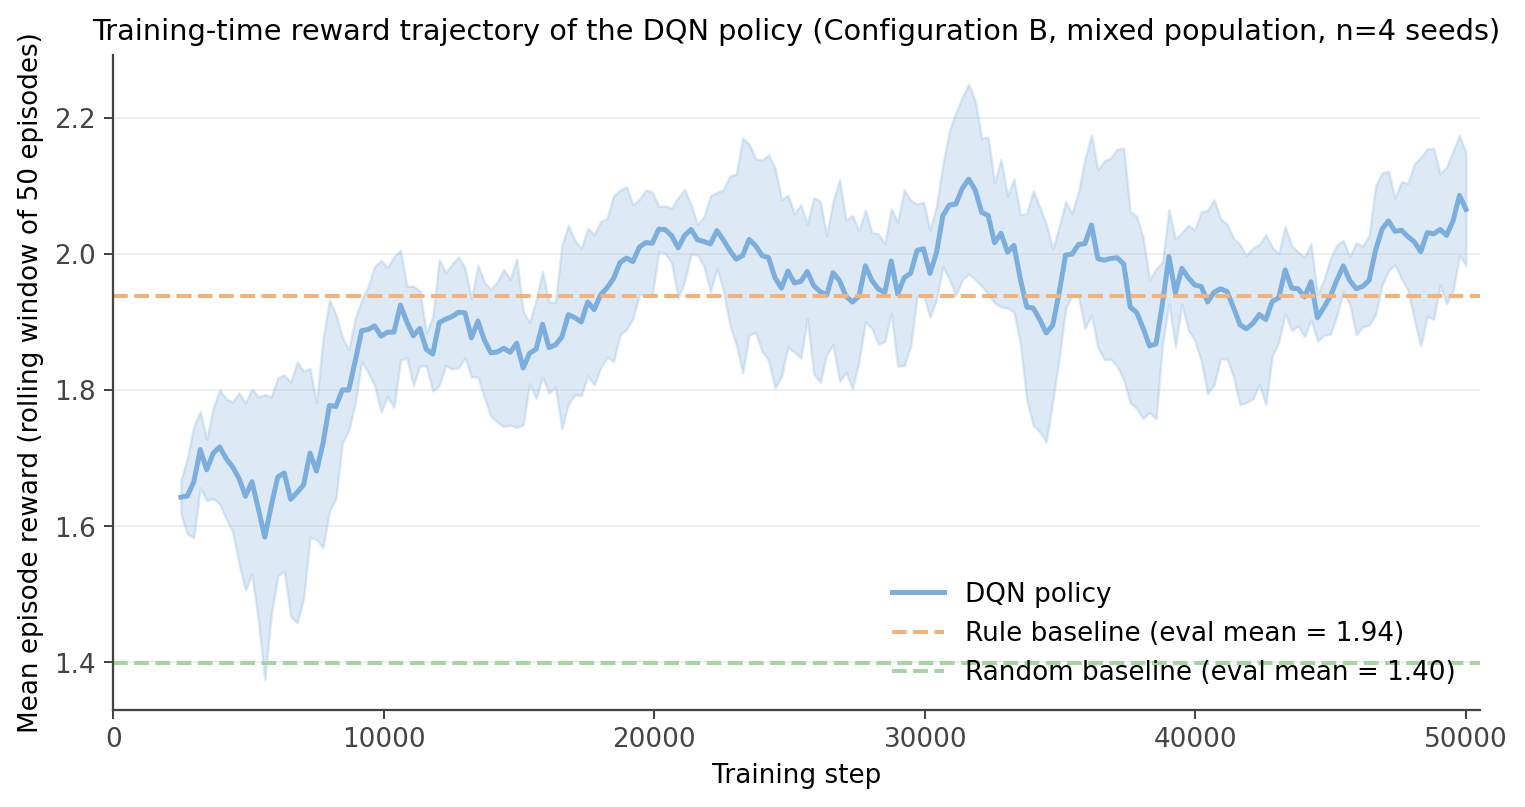
\includegraphics[width=0.95\textwidth]{Figures/rl_figA_learning_curve.png}
    \caption{Training-time reward trajectory of the \ac{DQN} policy
    on Configuration~B with the eval-time reward of the rule and
    random baselines as horizontal references. The confidence
    band is $\pm 1.96$ standard errors across four seeds. The
    rule and random baselines do not undergo training; their
    lines are the average evaluation reward of fixed policies
    and are shown as horizontal references so that the \ac{DQN}
    trajectory can be read against a stable benchmark.}
    \label{fig:rl_figA_learning_curve}
\end{figure}

\begin{figure}[H]
    \centering
    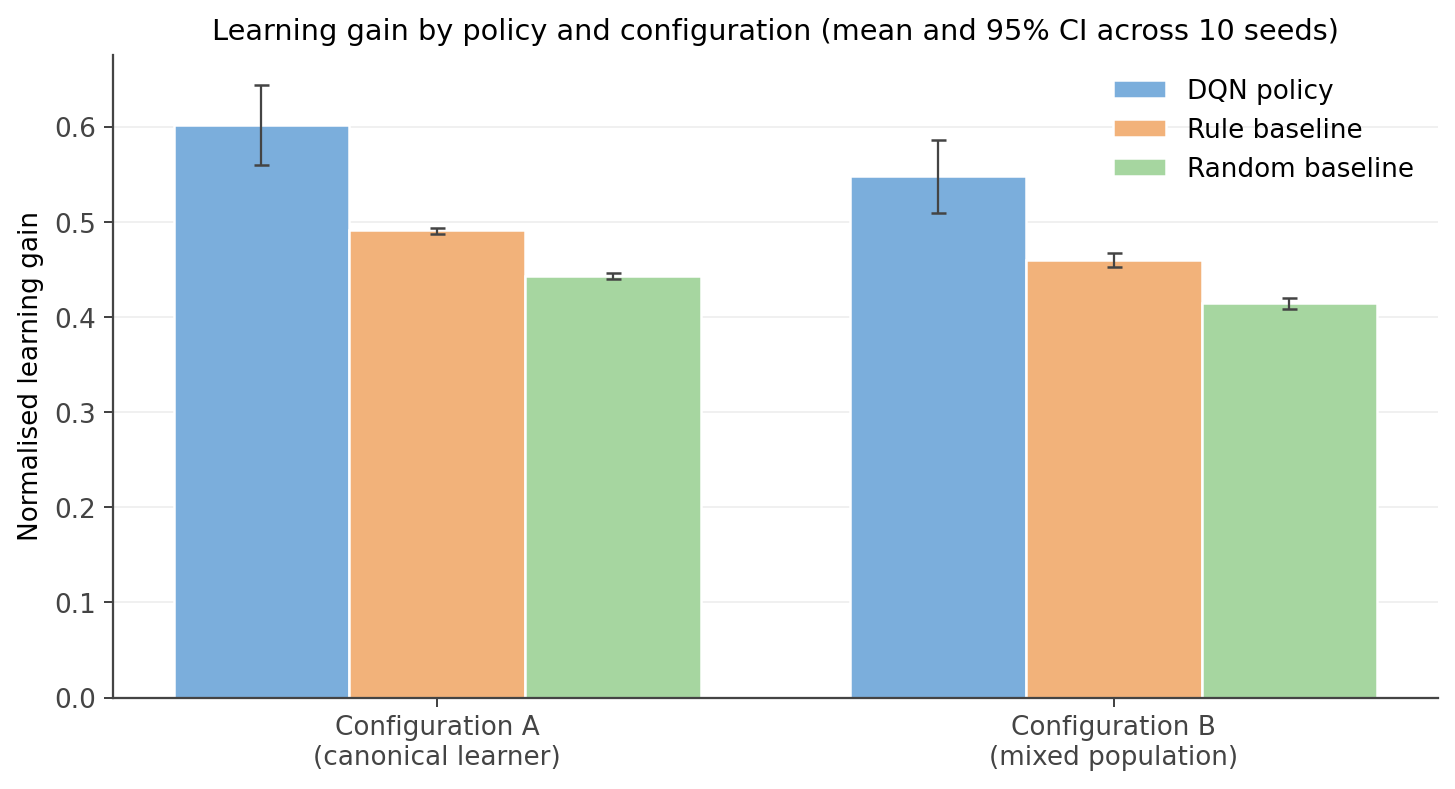
\includegraphics[width=0.95\textwidth]{Figures/rl_figB_learning_gain.png}
    \caption{Normalised learning gain by policy and
    configuration with $95\%$ bootstrap confidence intervals
    across ten seeds.}
    \label{fig:rl_figB_learning_gain}
\end{figure}

\begin{figure}[H]
    \centering
    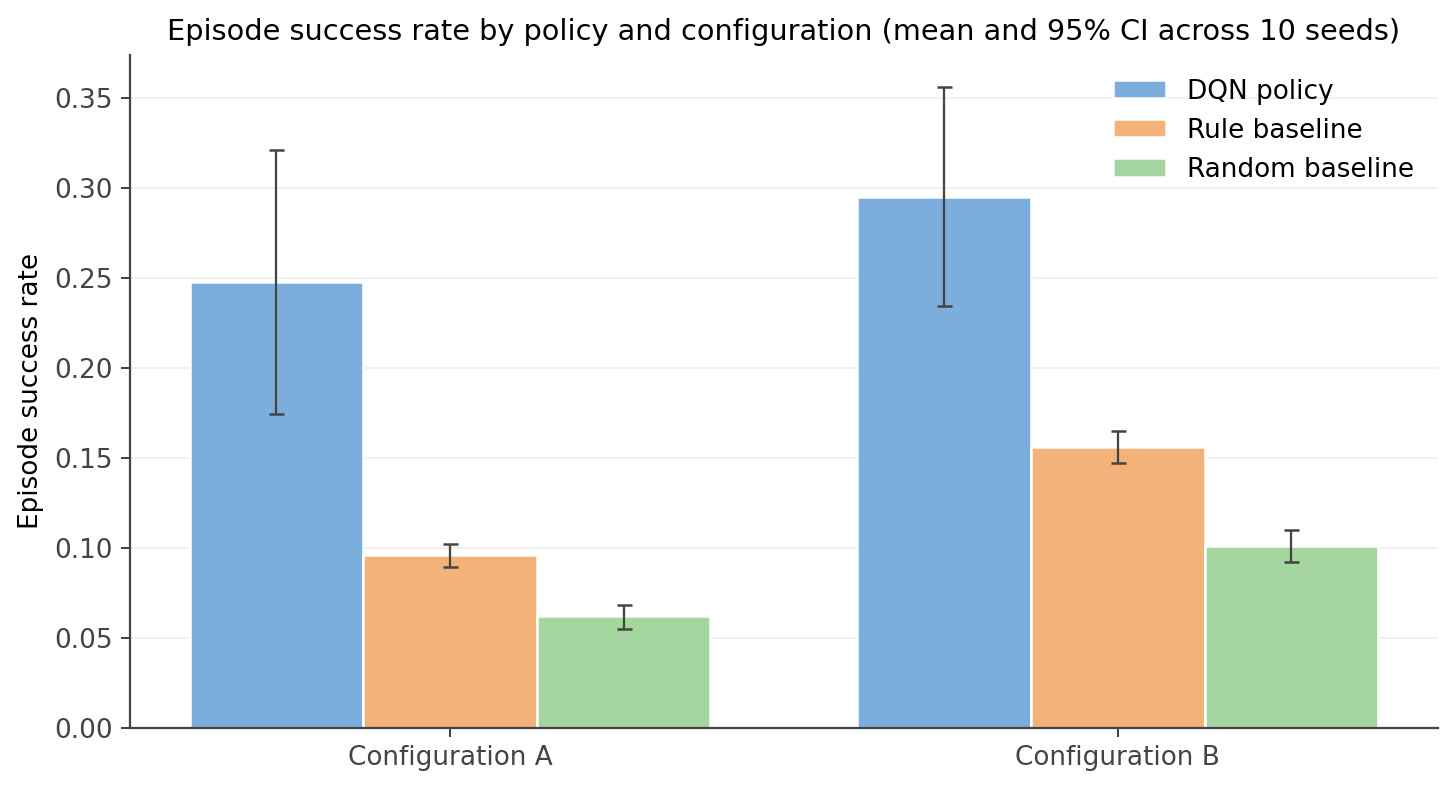
\includegraphics[width=0.95\textwidth]{Figures/rl_figC_success_rate.png}
    \caption{Episode success rate by policy and configuration
    with $95\%$ bootstrap confidence intervals across ten seeds.}
    \label{fig:rl_figC_success_rate}
\end{figure}

% ---------------------------------------------------------------
\subsection{Robustness and Generalisation}\label{sec:results_adapt_robustness}
% ---------------------------------------------------------------

Figure~\ref{fig:rl_figD_robustness} shows the per-seed
distribution of normalised learning gain. The standard
deviations across the ten seeds are $0.0679$ on Configuration~A
and $0.0614$ on Configuration~B, giving coefficients of
variation of $0.113$ and $0.112$. No seed produced a degenerate
policy, no evaluation episode terminated through
frustration-driven dropout, and the rolling-window training
reward never collapsed in any run.

\begin{figure}[H]
    \centering
    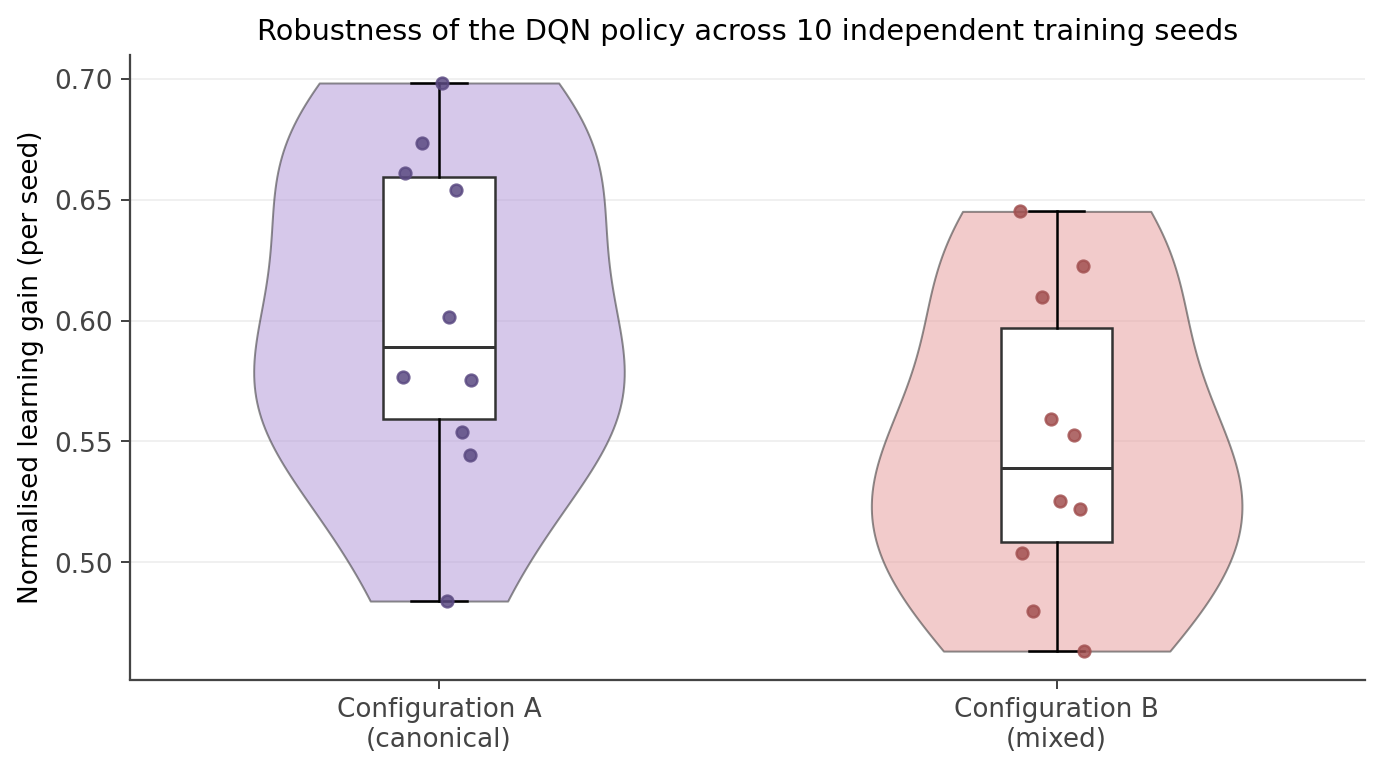
\includegraphics[width=0.80\textwidth]{Figures/rl_figD_robustness.png}
    \caption{Per-seed normalised learning gain for both
    configurations. Violin shapes show the empirical
    distribution; the inner box reports the median and
    interquartile range.}
    \label{fig:rl_figD_robustness}
\end{figure}

Generalisation behaviour separates the two configurations. The
canonical-trained policy reaches a same-population learning
gain of $0.602$ but its transfer learning gain on the mixed
population drops to $0.553$, a positive gap of $0.049$ in every
one of the ten seeds. The mixed-trained policy reaches
$0.548$ in-population, has a zero gap by construction, and
transfers upward to the canonical learner at $0.607$. The
canonical-only setting therefore overfits the simulator
personality, whereas mixed-population training trades a small
amount of in-distribution gain for distributionally robust
deployment behaviour \cite{dulacarnold_challenges_2021}. The
mixed-trained policy of Configuration~B is the recommended
thesis system.

% ---------------------------------------------------------------
\subsection{Comparison with Prior Studies}\label{sec:results_adapt_literature}
% ---------------------------------------------------------------

Cross-study numerical comparison across reinforcement-learning
intelligent tutoring systems is rarely meaningful. Studies
differ in their simulators, reward functions, state and action
spaces, learner and emotion models and evaluation protocols, so
equally numbered results do not measure the same quantity. The
comparison reported here is therefore qualitative and
architectural. Each prior system is positioned on the seven
design dimensions on which the present thesis takes a stance,
namely the use of \ac{DQN}, an educational or \ac{ITS} focus, synthetic
learners for training, knowledge modelling, emotion modelling,
\ac{RL}-driven adaptation and end-to-end perception-decision
integration. Table~\ref{tab:rl_prior_matrix} reports the
coverage matrix.

% Explicit RGB definitions so the markers work regardless of
% which xcolor mode the preamble loads.
\definecolor{matrixGreen}{RGB}{46,125,50}
\definecolor{matrixRed}{RGB}{198,40,40}
\definecolor{matrixAmber}{RGB}{230,140,0}
\providecommand{\yes}{\textcolor{matrixGreen}{$\checkmark$}}
\providecommand{\no}{\textcolor{matrixRed}{$\times$}}
\providecommand{\partialc}{\textcolor{matrixAmber}{$\sim$}}

\begin{table}[H]
\centering
\footnotesize
\caption{Component coverage of prior reinforcement-learning
intelligent tutoring systems on the seven design dimensions of
the present thesis. The first column reports bibliography
reference numbers; full bibliographic information is available
in the References section.
\textcolor{matrixGreen}{$\checkmark$} denotes that the
component is present and central,
\textcolor{matrixRed}{$\times$} that it is absent, and
\textcolor{matrixAmber}{$\sim$} that it is partial or
implicit.}
\label{tab:rl_prior_matrix}
\setlength{\tabcolsep}{4pt}
\renewcommand{\arraystretch}{1.45}
\begin{tabular}{cccccccc c}
\toprule
\textbf{Study} & \textbf{\ac{DQN}} & \textbf{Edu/} & \textbf{Synth.} & \textbf{Know.} & \textbf{Emo.} & \textbf{\ac{RL}} & \textbf{\ac{FER}--\ac{RL}} & \textbf{Cov.} \\
 & & \textbf{\ac{ITS}} & \textbf{stud.} & \textbf{mod.} & \textbf{mod.} & \textbf{adapt.} & \textbf{framework} & \\
\midrule
\cite{sanz_ausin_leveraging_2019}                       & \yes & \yes & \no       & \yes & \no       & \yes & \no       & 4/7 \\
\cite{abdelshiheed_bridging_2023}                       & \no  & \yes & \no       & \yes & \no       & \yes & \no       & 3/7 \\
\cite{kubotani_rltutor_2021}                            & \no  & \yes & \yes      & \yes & \no       & \yes & \no       & 4/7 \\
\cite{bassen_using_2020}                                & \no  & \yes & \yes      & \yes & \no       & \yes & \no       & 4/7 \\
\cite{fahid_online_2024}                                & \no  & \yes & \yes      & \yes & \no       & \yes & \no       & 4/7 \\
\cite{perez_emotions_2024}                              & \no  & \yes & \no       & \yes & \yes      & \yes & \no       & 4/7 \\
\cite{govea_implementation_2024}                        & \no  & \yes & \no       & \partialc & \yes & \yes & \no       & 4/7 \\
\cite{wang_dual_state_2024}                             & \no  & \yes & \no       & \yes & \yes      & \no  & \no       & 3/7 \\
\cite{sun_daskt_2025}                                   & \no  & \yes & \yes      & \yes & \yes      & \no  & \no       & 4/7 \\
\cite{axak_adaptive_2025}                               & \yes & \yes & \no       & \no  & \no       & \yes & \no       & 3/7 \\
\cite{noauthor_dqn-based_nodate}                        & \yes & \yes & \partialc & \yes & \no       & \yes & \no       & 4.5/7 \\
\midrule
\cite{guo_bridging_2026}                                & \yes & \yes & \no       & \yes & \partialc & \yes & \no       & 4.5/7 \\
\cite{sayed_ai-based_2023}                              & \yes & \yes & \no       & \yes & \partialc & \yes & \no       & 4.5/7 \\
\cite{Prabakaran2025FacialExpressionAdaptiveTeaching}   & \no  & \yes & \no       & \no  & \yes      & \yes & \partialc & 4/7 \\
\midrule
\textbf{Proposed \ac{FER}-\ac{RL} system (this thesis)}           & \yes & \yes & \yes      & \yes & \yes      & \yes & \yes      & \textbf{7/7} \\
\bottomrule
\end{tabular}
\end{table}

The matrix is to be read qualitatively. Three patterns emerge.
First, prior systems cluster into two largely disjoint groups:
deep value-based controllers without an affective channel
\cite{sanz_ausin_leveraging_2019,abdelshiheed_bridging_2023,
kubotani_rltutor_2021,bassen_using_2020,fahid_online_2024,
axak_adaptive_2025,noauthor_dqn-based_nodate} and affect-aware
models that integrate emotion information either without a deep
value-based controller or without a closed-loop \ac{RL} adaptation
\cite{perez_emotions_2024,govea_implementation_2024,
wang_dual_state_2024,sun_daskt_2025,
Prabakaran2025FacialExpressionAdaptiveTeaching}. The thesis
sits at the intersection of the two groups. Second, the most
recent emotion-aware \ac{DQN} systems
\cite{sayed_ai-based_2023,guo_bridging_2026} extend value-based
control with an affective input, but the affective signal is
treated as a labelled input rather than as the output of a
perception layer evaluated on a public benchmark; the studies
indicated by $\sim$ in the emotion column include emotion in the
state representation without validating a perception pipeline on
a standard dataset. The thesis evaluates the \ac{FER} perception
layer on \ac{DAiSEE} in Section~\ref{sec:results_fer} and integrates
the resulting affect vector with the decision layer through a
documented interface, which is the principal differentiator on
the integration column. Third, no numerical advantage is claimed
against the entries in Table~\ref{tab:rl_prior_matrix} because
the simulators and reward functions differ across studies; the
contribution is the joint coverage of all seven dimensions
rather than a numerical ranking on any single dimension.

% ---------------------------------------------------------------
\subsection{Discussion and Educational Interpretation}\label{sec:results_adapt_discussion}
% ---------------------------------------------------------------

Three findings drive the discussion.

\paragraph{The \ac{DQN} policy outperformed both baselines.} The
learned policy improved on the rule-based expert by an absolute
learning gain of $0.088$ on Configuration~B ($d=2.01$) and on
the random policy by an absolute learning gain of $0.134$
($d=3.05$); the same ordering holds on every outcome metric
and in both populations. The interpretation is that
value-based control integrates cognitive and affective signals
into a multi-step return more effectively than a hand-crafted
heuristic or unstructured sampling. The result is consistent
with prior reports that affect-aware controllers outperform
rule-based tutors when the reward couples knowledge and affect
\cite{sayed_ai-based_2023,
Prabakaran2025FacialExpressionAdaptiveTeaching}.

\paragraph{Mixed-population training improved robustness and
transferability.} Configuration~A reaches the higher in-
population learning gain ($0.602$ vs $0.548$) but transfers
downward to mixed dynamics in every seed (mean gap $+0.049$).
Configuration~B has a zero in-distribution gap by construction
and transfers upward to the canonical learner ($0.607$). The
policy that experienced heterogeneous learners during training
generalises more credibly to the heterogeneous populations that
classrooms produce, in line with the heterogeneous-learner
adaptation literature
\cite{ihichr_systematic_2024,zerkouk_comprehensive_2025} and the
real-world \ac{RL} framing of generalisation
\cite{dulacarnold_challenges_2021}.

\paragraph{Policy behaviour reflected affect-aware adaptation
rather than static instruction.} The affect-conditioned action
distribution of the \ac{DQN} policy
(Figure~\ref{fig:rl_figE_policy_heatmap}) selects scaffold on
$90\%$ of confused states, harder problem on $99\%$ of bored
states, encouragement on $74\%$ of frustrated states and a
scaffold-plus-no-action mixture under engagement. Two actions,
scaffold ($31.7\%$) and harder problem ($45.6\%$), dominate the
population-level distribution; the remaining six actions appear
as state-conditional refinements rather than as collapsed or
uniform behaviour. The action heatmap aligns with the
zone-of-proximal-development principle used by \ac{DQN}-based
cognitive-load tutors \cite{sayed_ai-based_2023} and with the
affect-aware \ac{ITS} prescription that scaffolding follows
confusion and motivational support follows frustration
\cite{woolf_affect-aware_2009,dmello_integrating_2005}. The
Control-Value framing of academic emotions
\cite{pekrun_control-value_2006} interprets the pattern as
control restoration under negative affect and value
maintenance under positive affect.

\begin{figure}[H]
    \centering
    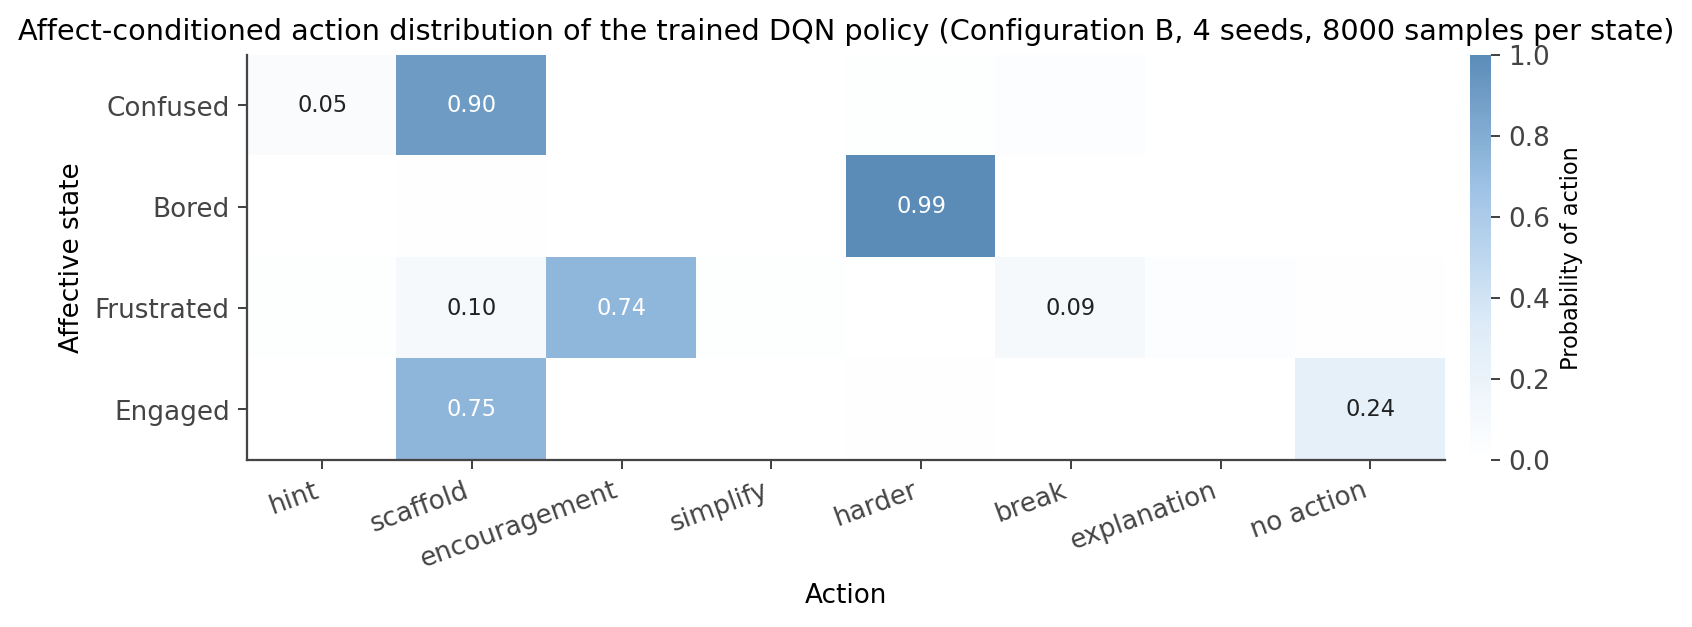
\includegraphics[width=0.95\textwidth]{Figures/rl_figE_policy_heatmap.png}
    \caption{Affect-conditioned action distribution of the
    trained \ac{DQN} policy on Configuration~B. Each row sums to one before omission; entries below 0.05 are hidden.}
    \label{fig:rl_figE_policy_heatmap}
\end{figure}

% ---------------------------------------------------------------
\subsection{\ac{FER}-\ac{RL} System Integration}\label{sec:results_adapt_ferrl}
% ---------------------------------------------------------------

Figure~\ref{fig:rl_figF_pipeline} illustrates the integrated
pipeline as a single control loop. The \ac{FER} module of Part~I is
the perception layer: at each interaction window it consumes
the face-aligned frames and emits a four-channel affect vector
$\mathbf{a}_t \in \{0,1\}^4$ over the labels boredom,
engagement, confusion and frustration. The \ac{RL} module of
Part~II is the decision layer: at each step it consumes the
six-dimensional learner state $\mathbf{s}_t$ and emits a
pedagogical action from the action set $\mathcal{A}$. The
continuous channels of $\mathbf{a}_t$ enter $\mathbf{s}_t$
directly; the \texttt{FERAdapter} interface projects the same
vector onto the discrete emotion identifier used for masking.
The same interface is used in simulator mode and in real-\ac{FER}
mode, with only the source of $\mathbf{a}_t$ changing.

\begin{figure}[H]
    \centering
    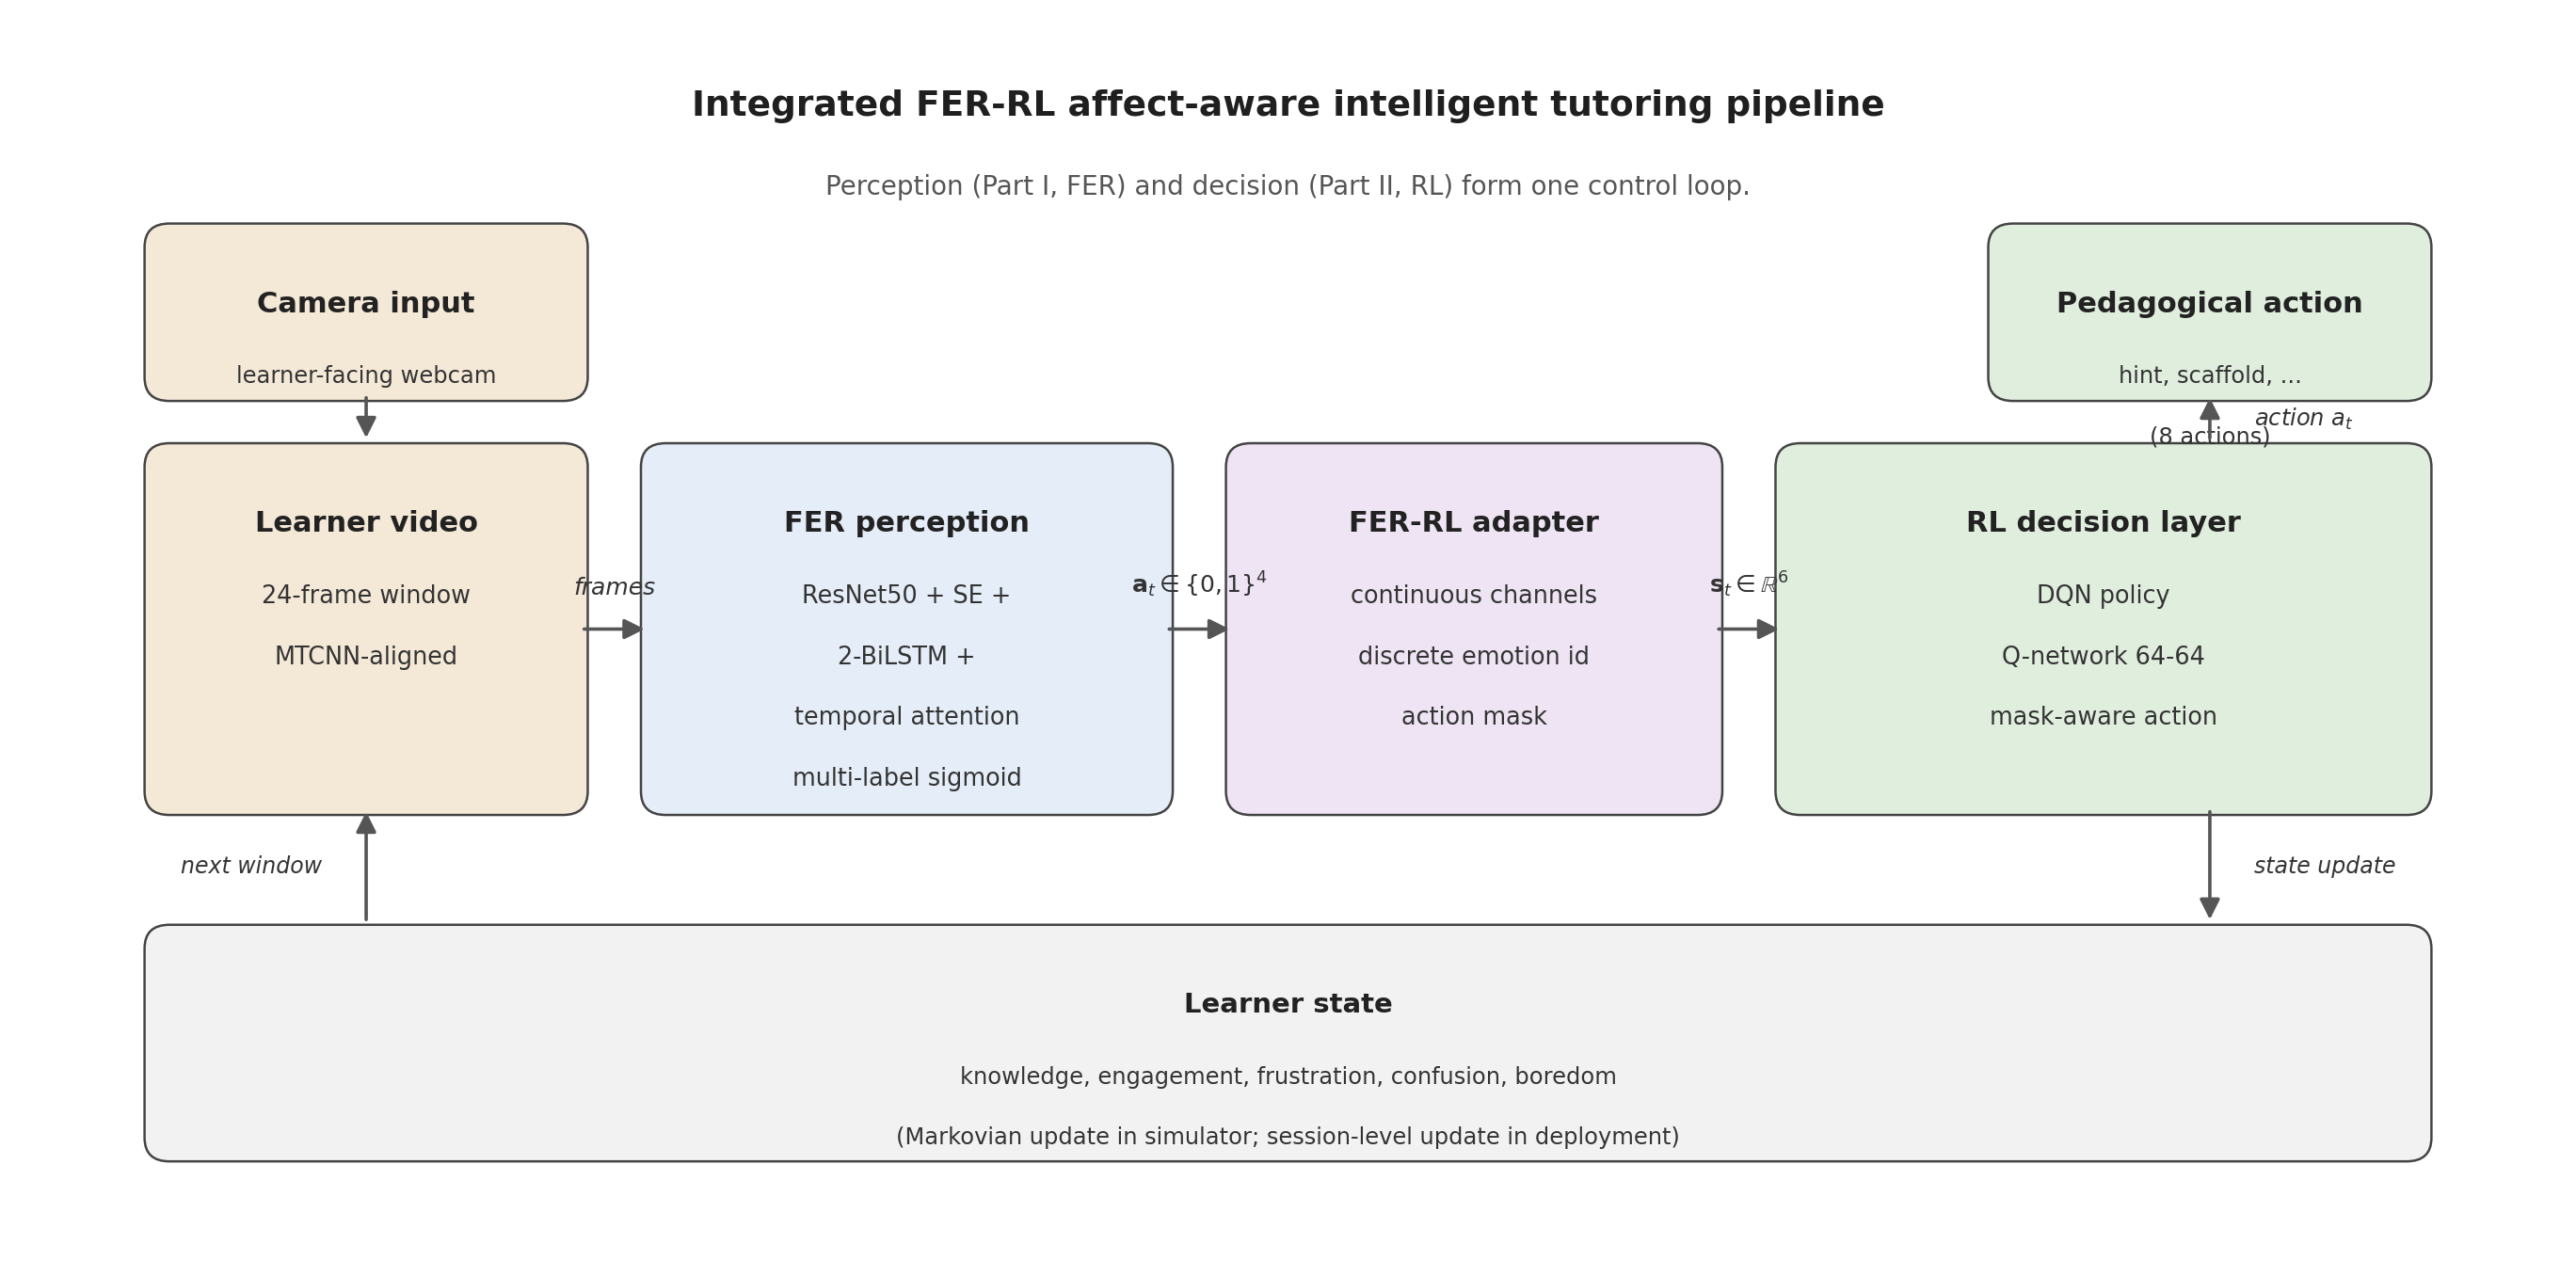
\includegraphics[width=0.98\textwidth]{Figures/rl_figF_fer_rl_pipeline_2.png}
    \caption{Integrated \ac{FER}-\ac{RL} pipeline. The perception layer
    converts a face-aligned window into a four-channel affect
    vector; the adapter assembles the \ac{RL} state; the \ac{DQN} policy
    emits a pedagogical action that updates the learner state at
    the next interaction step.}
    \label{fig:rl_figF_pipeline}
\end{figure}

The operational dependency is asymmetric. The decision layer
cannot act without affect information, so a failure of the \ac{FER}
module collapses the system to a state-independent policy. The
perception layer in turn has no mechanism for changing the
learner's affect; without the decision layer it remains a
diagnostic instrument. The two modules are therefore halves of
one control loop and the quantitative findings of Part~I and
Part~II jointly characterise the system. The reliability
profile of the perception layer reported in
Section~\ref{sec:results_fer_overall} (engagement F1 $0.975$;
minority-label F1 between $0.224$ and $0.358$) defines the
operating condition under which the decision layer must
function in deployment, and the action mask of the simulator
guarantees that catastrophic actions remain inadmissible
regardless of perception noise. Educator oversight of the
mask, as advocated by \cite{calo2024educatordriven}, and the
privacy and integration considerations summarised by
\cite{vistorte_integrating_2024}, complete the deployment
envelope of the integrated architecture.

% ---------------------------------------------------------------
\subsection{Adaptation Module Summary}\label{sec:results_adapt_summary}
% ---------------------------------------------------------------

\begin{itemize}
\item The \ac{DQN} policy outperforms the rule-based expert and the
random baseline on every outcome metric (learning gain, mean
reward, success rate) and in both student populations, with
Cohen's $d$ between $1.81$ and $3.30$ and Holm-corrected
$p$-values below $10^{-2}$.
\item Convergence is reproducible across the ten seeds
(coefficient of variation $0.112$ on Configuration~B), and no
evaluation episode terminated through frustration-driven
dropout.
\item Mixed-population training transfers upward to the
canonical learner and shows no overfitting signal, whereas
canonical-only training overfits in every seed (mean gap
$+0.049$); the mixed-trained policy of Configuration~B is the
recommended deployment configuration.
\item Affect-conditioned action selection is concentrated and
pedagogically interpretable, with scaffold and harder problem
as the dominant actions and the remaining six actions appearing
as state-conditional refinements.
\end{itemize}

% =====================================================================
% UNIFIED CHAPTER SUMMARY
% =====================================================================
\section{Chapter Summary}\label{sec:results_chapter_summary}

This chapter has reported the evaluation of the two modules
that together constitute the affect-aware intelligent tutoring
system defended in this thesis. The findings of Part~I
(perception, Section~\ref{sec:results_fer}) and Part~II
(decision, Section~\ref{sec:results_adapt_part}) are
summarised below.

\begin{itemize}
\item \textbf{Perception layer.} The proposed ResNet50 with \ac{SE}
block, two-layer \ac{BiLSTM} and temporal attention reaches Macro F1
$0.453$, Weighted F1 $0.798$, Micro F1 $0.724$ and Samples F1
$0.746$ on the \ac{DAiSEE} test split under the standardised
pipeline, with per-label F1 of $0.975$ on engagement, $0.358$
on boredom, $0.255$ on frustration and $0.224$ on confusion.
\item \textbf{Decision layer.} The \ac{DQN} policy is the highest-
scoring policy on every outcome metric and in both student
populations. The mixed-population policy of Configuration~B
reaches learning gain $0.548$, mean reward $2.031$ and success
rate $0.295$.
\item \textbf{Effect magnitude.} The advantage over the rule
and random baselines is large by Cohen's convention ($d$
between $1.81$ and $3.30$) and statistically significant at
$p_{\text{Holm}}<10^{-2}$ on every pairwise test.
\item \textbf{Robustness and generalisation.} The policy
converges reproducibly across ten seeds, avoids
frustration-driven dropout and selects actions that vary with
the affective state. Mixed-population training transfers upward
to the canonical learner and is the recommended deployment
configuration.
\item \textbf{Integrated architecture.} The \ac{FER} perception
layer and the \ac{DQN} decision layer form one closed control loop:
the \ac{FER} module supplies the affect vector $\mathbf{a}_t$, the
adapter assembles the \ac{RL} state, the \ac{DQN} policy emits a
pedagogical action and the action updates the learner state at
the next interaction step. Together they realise an
affect-aware adaptive tutoring system in which perception and
decision act as complementary halves of a single architecture.
\end{itemize}
